\documentclass{beamer}
 
\usepackage[utf8]{inputenc}
\usepackage{braket}
\usepackage{mathtools} % Needed for \prescript
\usetheme{Boadilla}
\setbeamertemplate{navigation symbols}{}
\usepackage{subfig}
\usepackage{hyperref}

\captionsetup[subfigure]{labelformat=empty}
\captionsetup[figure]{labelformat=empty}

\newcommand{\tot}{\mathrm{tot}}
\DeclareMathOperator{\Tr}{Tr}

%Information to be included in the title page:
\title{LSTM Tagger}
\author{Philipp Windischhofer}
%\institute{ETH Zürich}
\date{\today}
  
\begin{document}
 
\frame{\titlepage}

%\begin{frame}
%\frametitle{Table of Contents}
%\tableofcontents
%\end{frame}

\begin{frame}
  \frametitle{The Setup}

  \begin{block}{Goal}
    Train a binary neural-network based classifier that can distinguish between $b$- and non-$b$-jets, using the raw jet data as input.
  \end{block}

  \begin{itemize}
  \item use \textsl{tracks} as the primary source of information
  \item number of tracks is unknown a-priori $\rightarrow$ cannot use an architecture that expects a fixed number of inputs
  \item currently looking into recurrent neural networks / LSTM networks
  \end{itemize}
\end{frame}

\begin{frame}
  \frametitle{LSTM-Networks}

  A special kind of recurrent neural network with a more complex internal structure...
  
  \begin{figure}[htb]
    \centering
    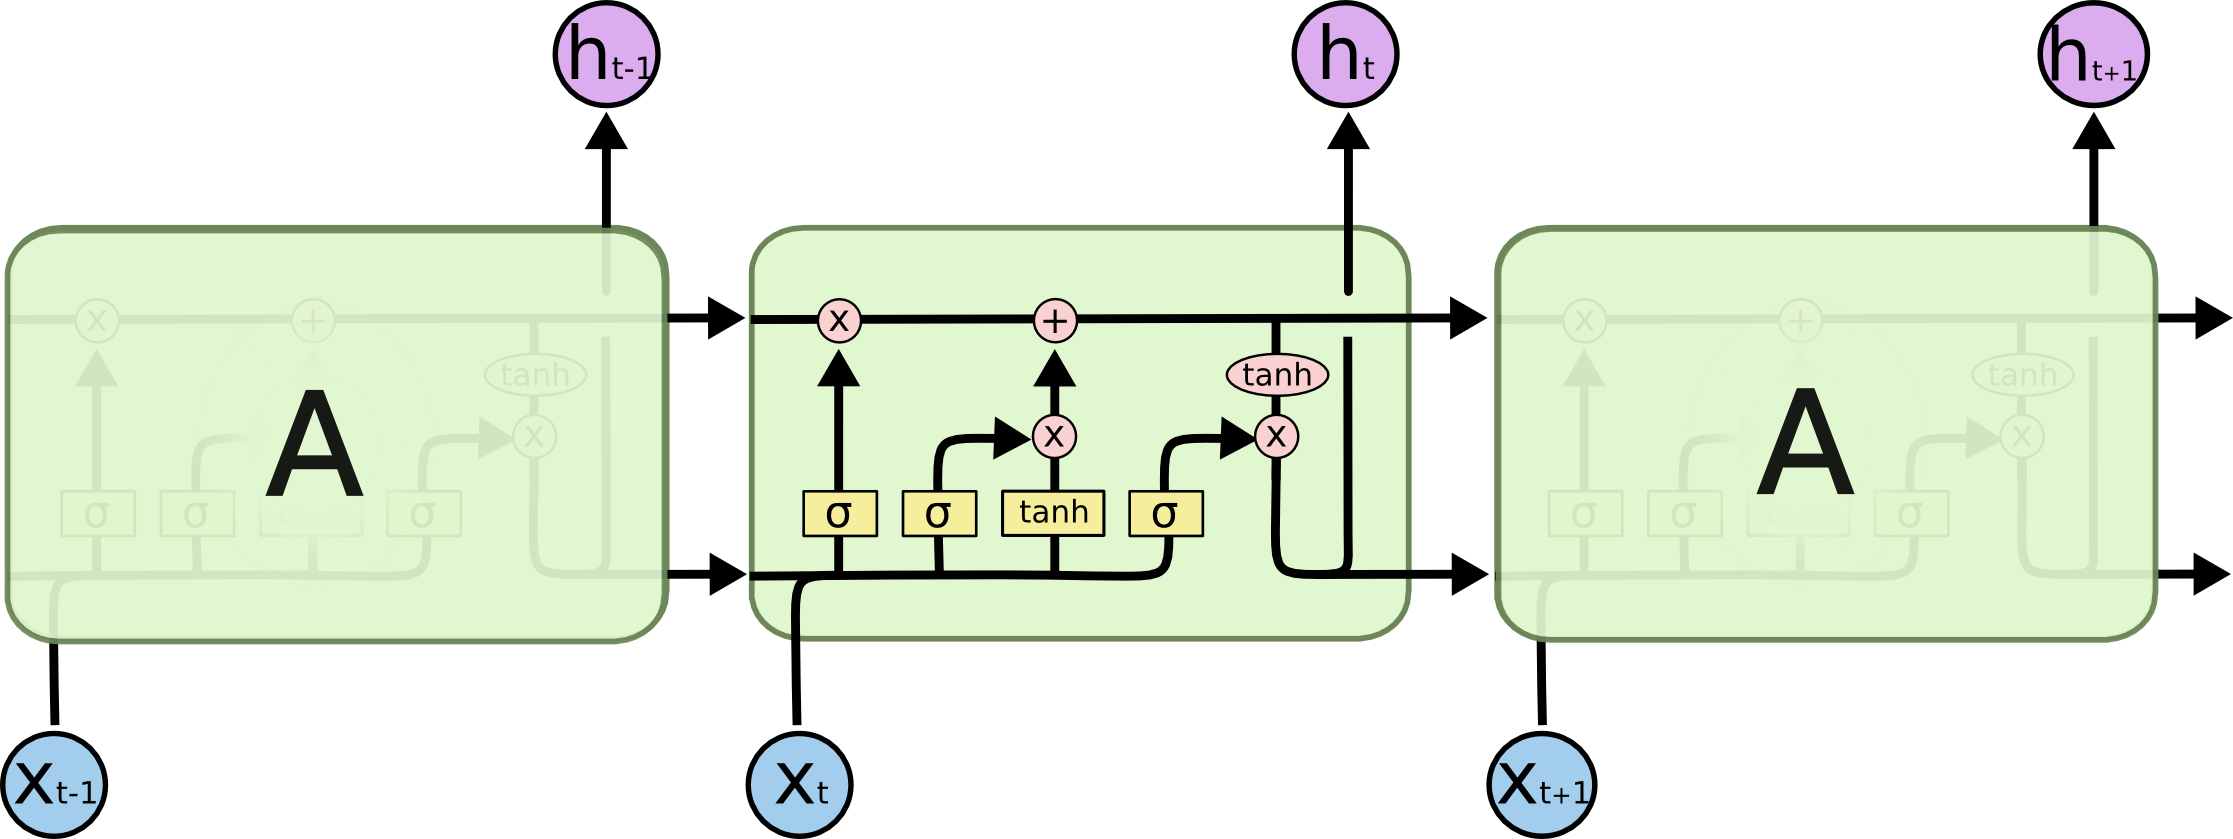
\includegraphics[width =0.88\textwidth]{LSTM3-chain.png}
    \caption{see \hyperlink{http://colah.github.io/posts/2015-08-Understanding-LSTMs/}{http://colah.github.io/posts/2015-08-Understanding-LSTMs/}}
  \end{figure}
    
\end{frame}

\begin{frame}
  \frametitle{The Workflow}
  \framesubtitle{Training}
  \begin{itemize}
  \item match tracks to their associated jets (contained in different ROOT trees)
  \item for each track in the jet, feed all 8 available track parameters into the classifier network during training
    \begin{itemize}
      \item use $p_T$ ordering, i.e.~hardest track first
    \end{itemize}
  \item supervised training: provide a binary (0/1) output value for each jet (from MC truth)
  \end{itemize}

  Now running on Piz Daint:
  \begin{itemize}
  \item roughly 2-3 $\times$ improvement in execution speed compared to PSI/Tier-3
  \item limited by Jet-Track-matching, which is handled by the CPU
  \item possible workaround: train multiple classifiers during the same run ``in parallel''
  \end{itemize}
\end{frame}

\begin{frame}
  \frametitle{The Workflow}
  \framesubtitle{Evaluation}
  \begin{itemize}
  \item compare performance to cMVA tagger as ``gold-standard''
  \item obtain ROC curves for both classifiers, correlation plots of the outputs
  \item currently: validation data is disjoint from training data, but from the same MC-run (i.e.~contains a similar event signature)
  \end{itemize}

\end{frame}

\begin{frame}
  \frametitle{Results so far}
  \begin{itemize}
  \item trained a number of LSTM networks, scanned the hyperparameters:
    \begin{itemize}
    \item number of nodes in each layer
    \item number of layers
    \item number of training epochs
    \end{itemize}
  \end{itemize}
  
  Details of the training:
  \begin{itemize}
  \item read training data in chunks of 10k jets
  \item use 8k jets for training, 2k jets to monitor performance during each epoch
  \end{itemize}
\end{frame}

\begin{frame}
  \frametitle{64 nodes / layer, 1 layer}

    \begin{figure}[htb]
    \centering
    \subfloat[][]{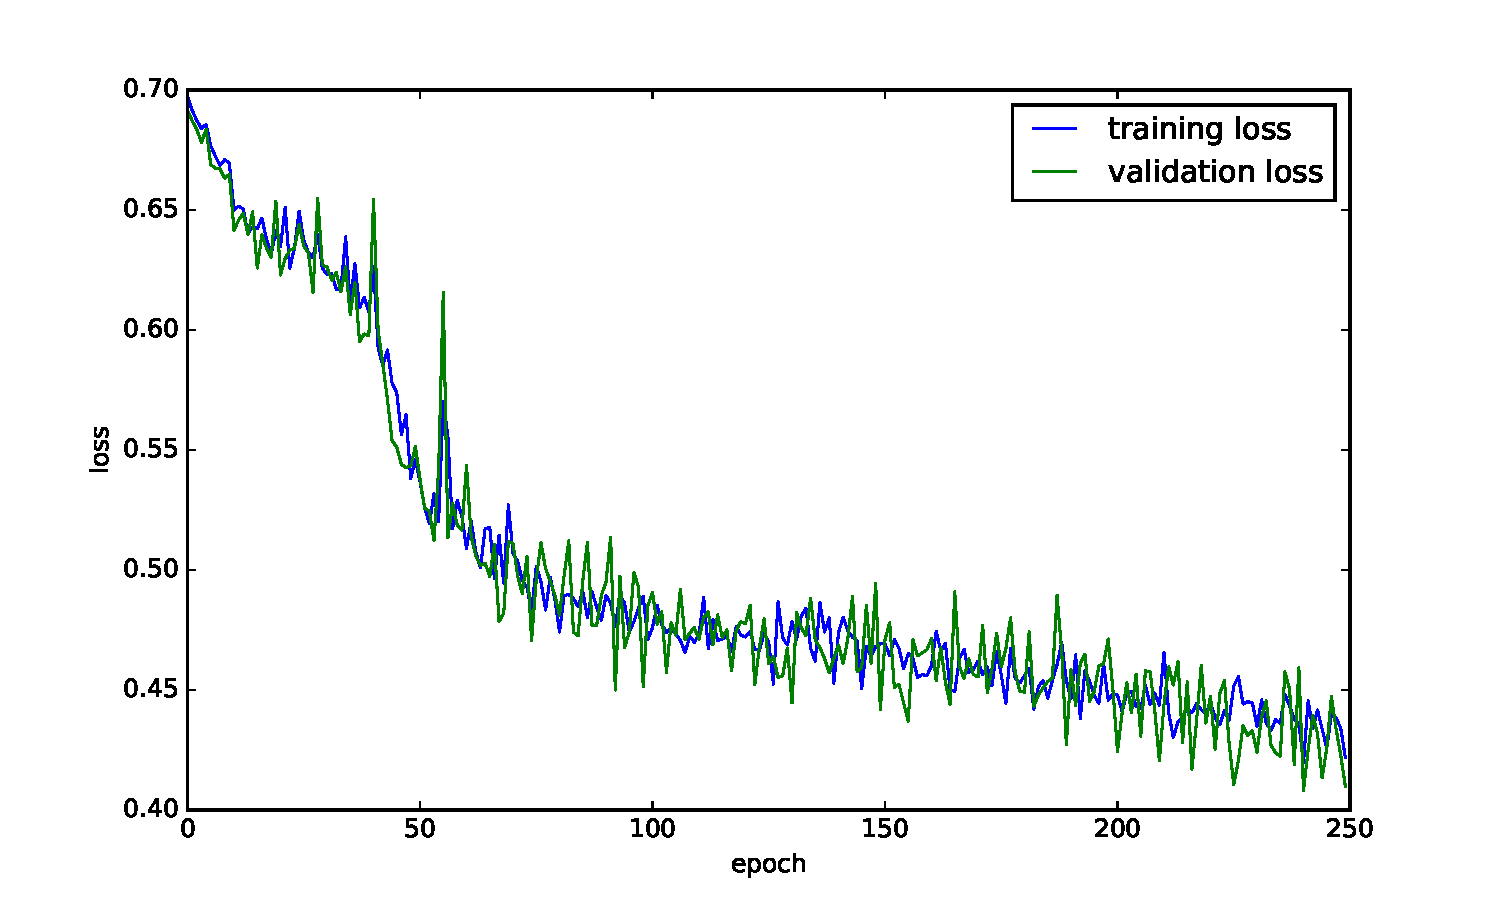
\includegraphics[width =0.5\textwidth]{../RNN_out/lstm64_1layer_singlestep_250/loss-history.pdf}}	
    \subfloat[][]{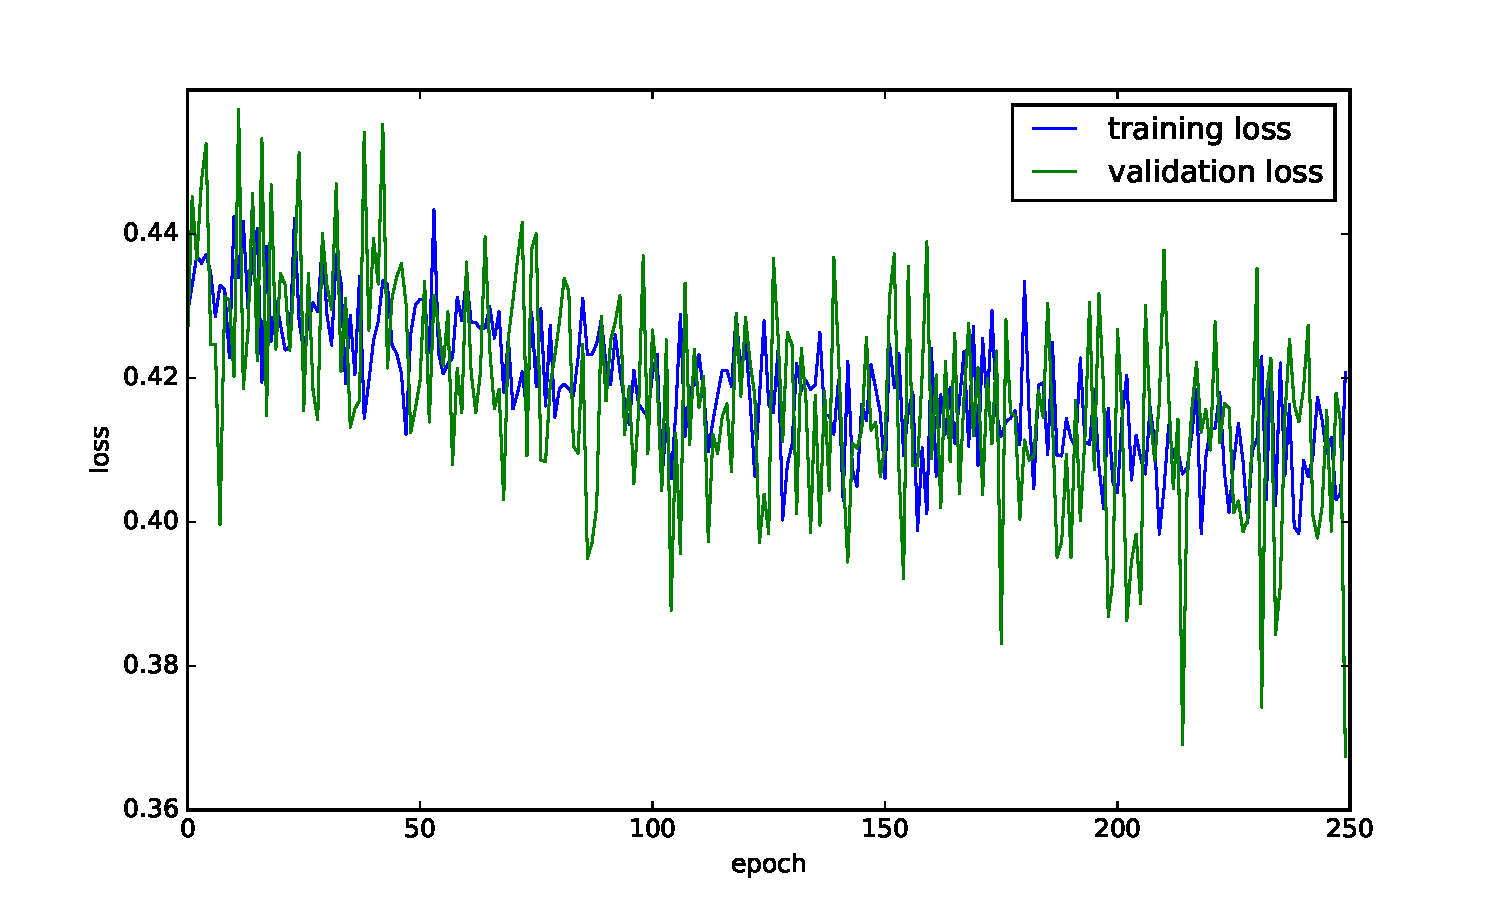
\includegraphics[width =0.5\textwidth]{../RNN_out/lstm64_1layer_singlestep_250_2/loss-history.pdf}}

    \caption{Loss function (binary cross-entropy) for epochs 1-250 (left) and 250-500 (right).}
  \end{figure}

\end{frame}

\begin{frame}
  \frametitle{64 nodes / layer, 1 layer}
    \begin{figure}[htb]
    \centering
    \subfloat[][]{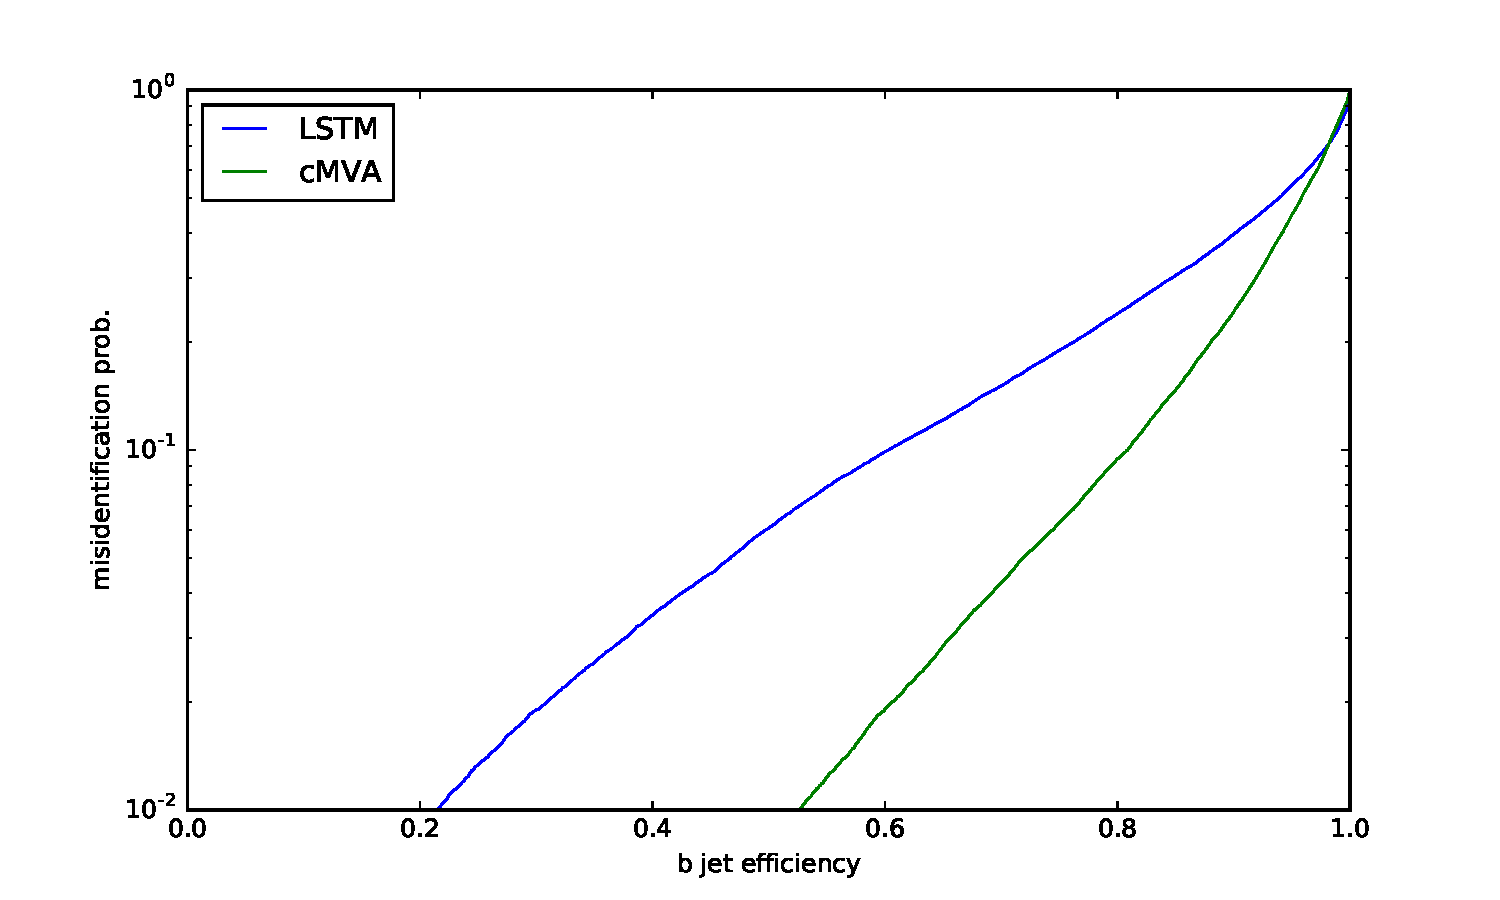
\includegraphics[width =0.5\textwidth]{../RNN_out/lstm64_1layer_singlestep_250/ROC-plot.pdf}\label{a}}	
    \subfloat[][]{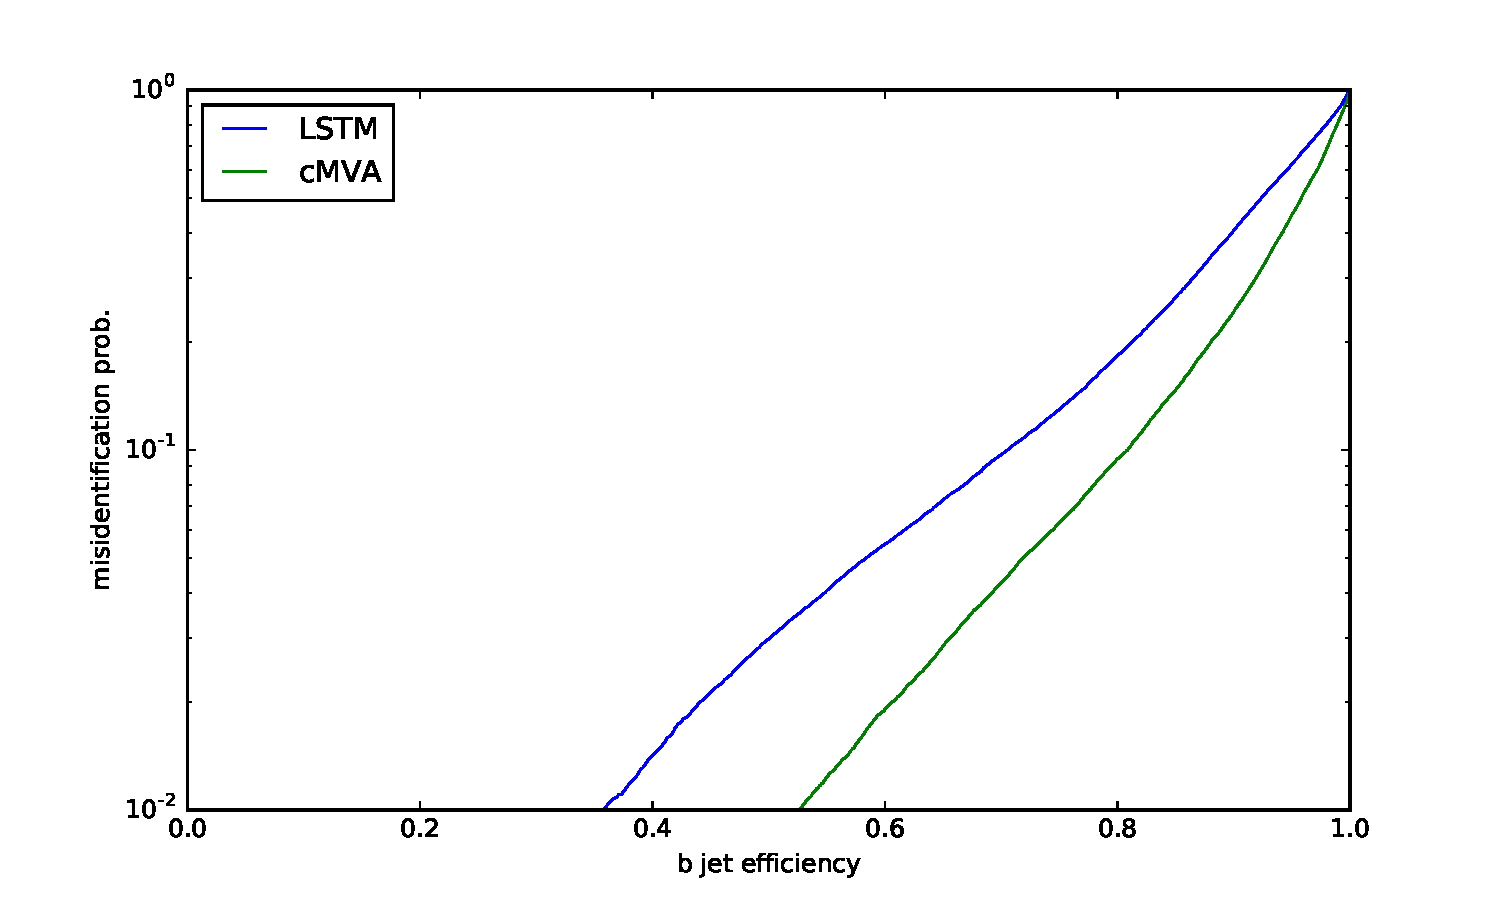
\includegraphics[width =0.5\textwidth]{../RNN_out/lstm64_1layer_singlestep_250_2/ROC-plot.pdf}\label{b}}

    \caption{ROC after 250 (left) and 500 training epochs (right) in comparison with the cMVA tagger.}
    \end{figure}

  Area under curve:
  \begin{itemize}
  \item AUC(cMVA) = 0.9233
  \item AUC(LSTM) = 0.8794
  \end{itemize}

\end{frame}

\begin{frame}
  \frametitle{64 nodes / layer, 3 layers}

  \begin{figure}[htb]
    \centering
    \subfloat[][]{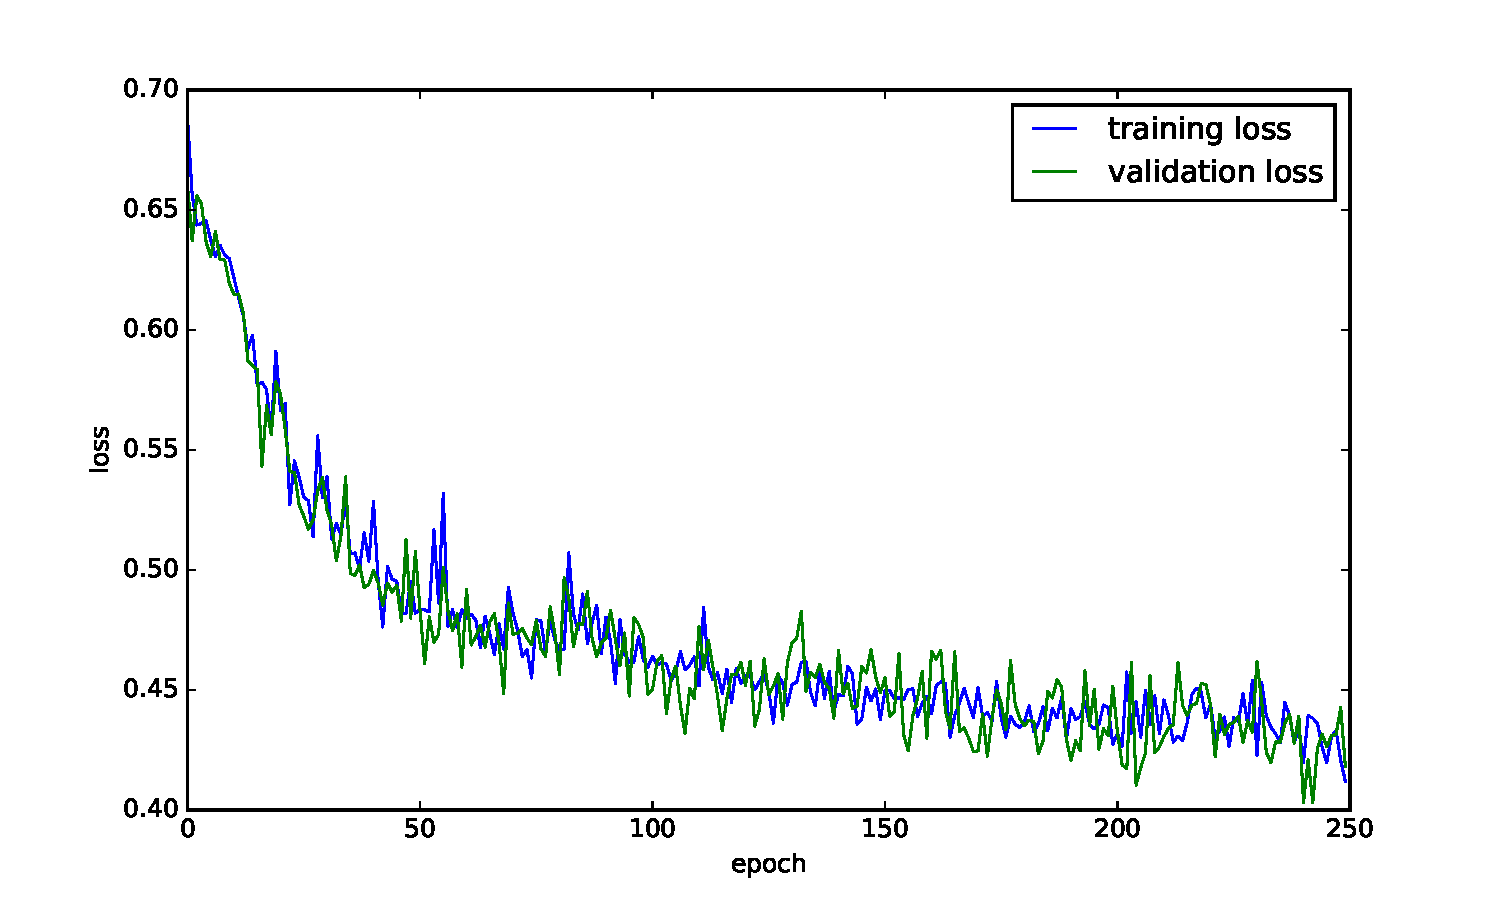
\includegraphics[width =0.5\textwidth]{../RNN_out/lstm64_3layers_singlestep_250/loss-history.pdf}\label{a}}
    \subfloat[][]{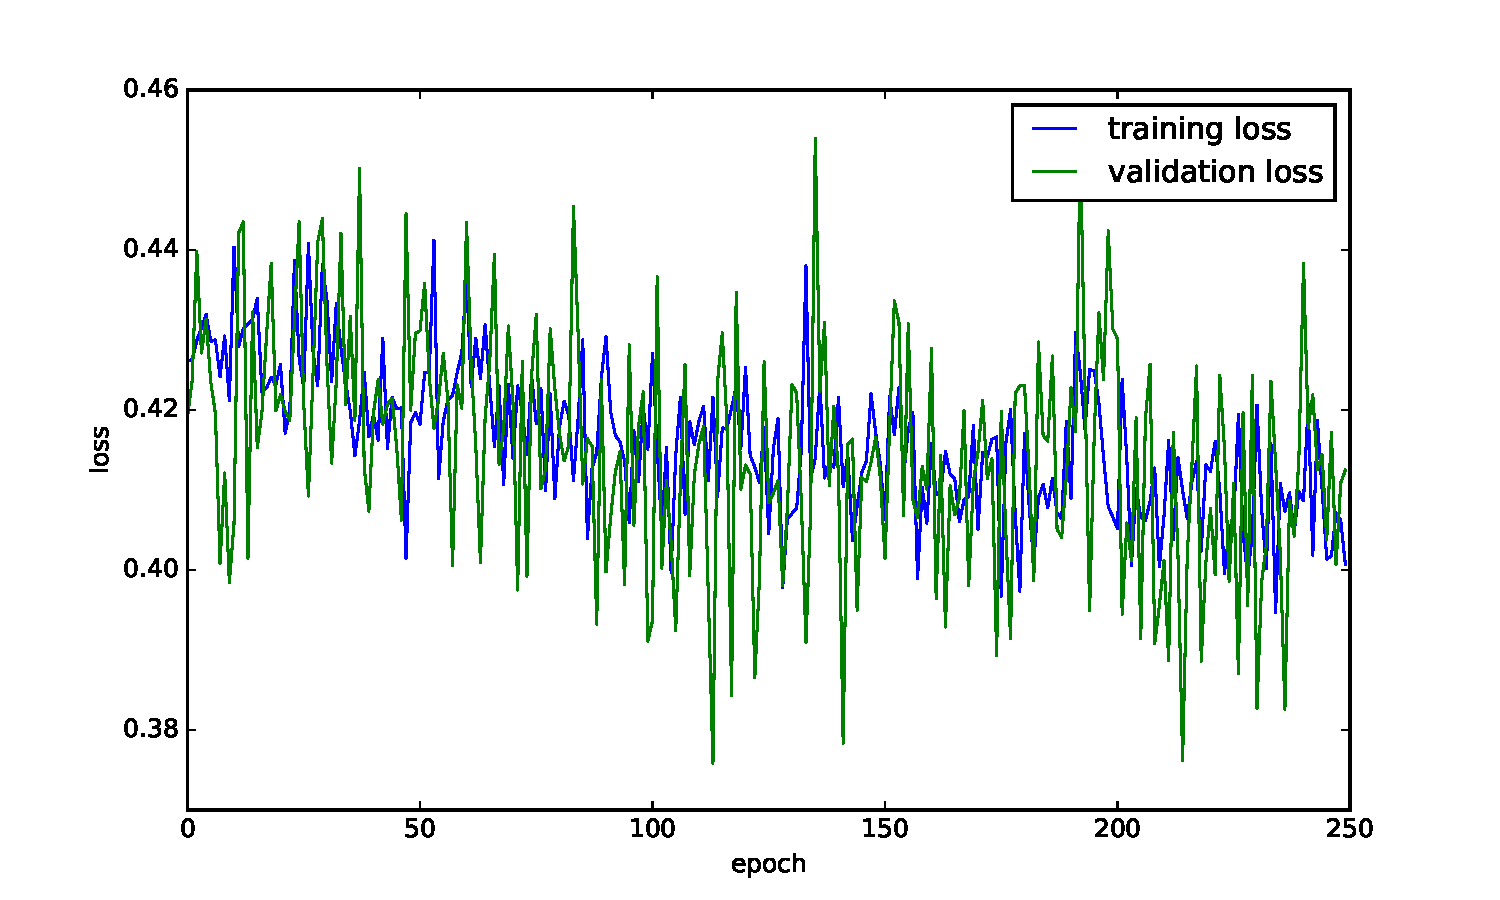
\includegraphics[width =0.5\textwidth]{../RNN_out/lstm64_3layers_singlestep_250_2/loss-history.pdf}\label{a}}	
    \caption{Loss function (binary cross-entropy) for epochs 1-250 (left) and 250-500 (right).}
  \end{figure}

\end{frame}

\begin{frame}
  \frametitle{64 nodes / layer, 3 layers}

  \begin{figure}[htb]
    \centering
    \subfloat[][]{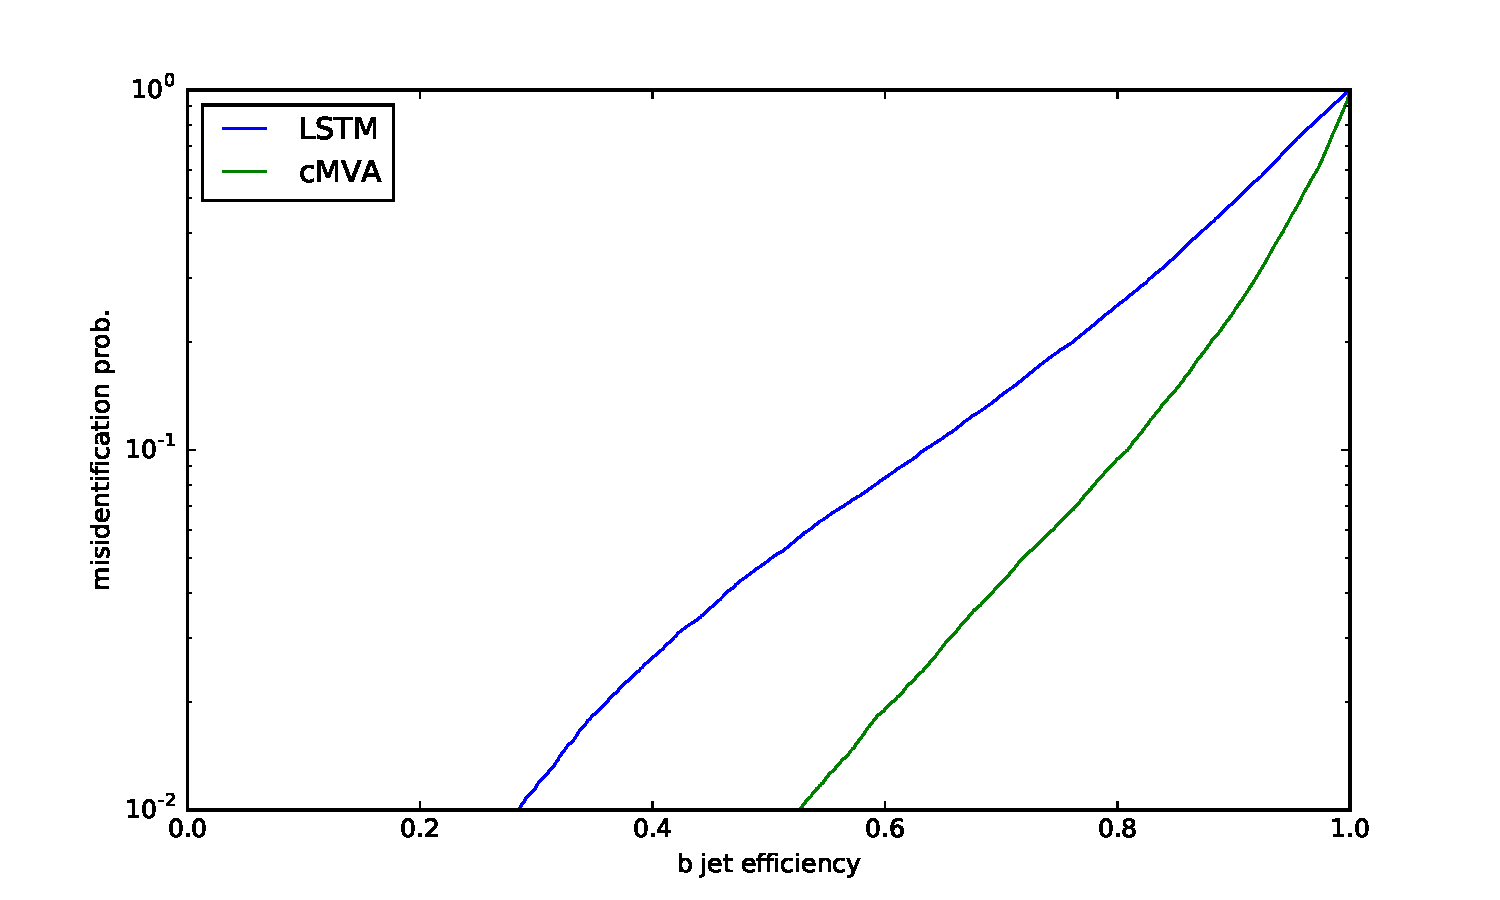
\includegraphics[width =0.5\textwidth]{../RNN_out/lstm64_3layers_singlestep_250/ROC-plot.pdf}\label{a}}	
    \subfloat[][]{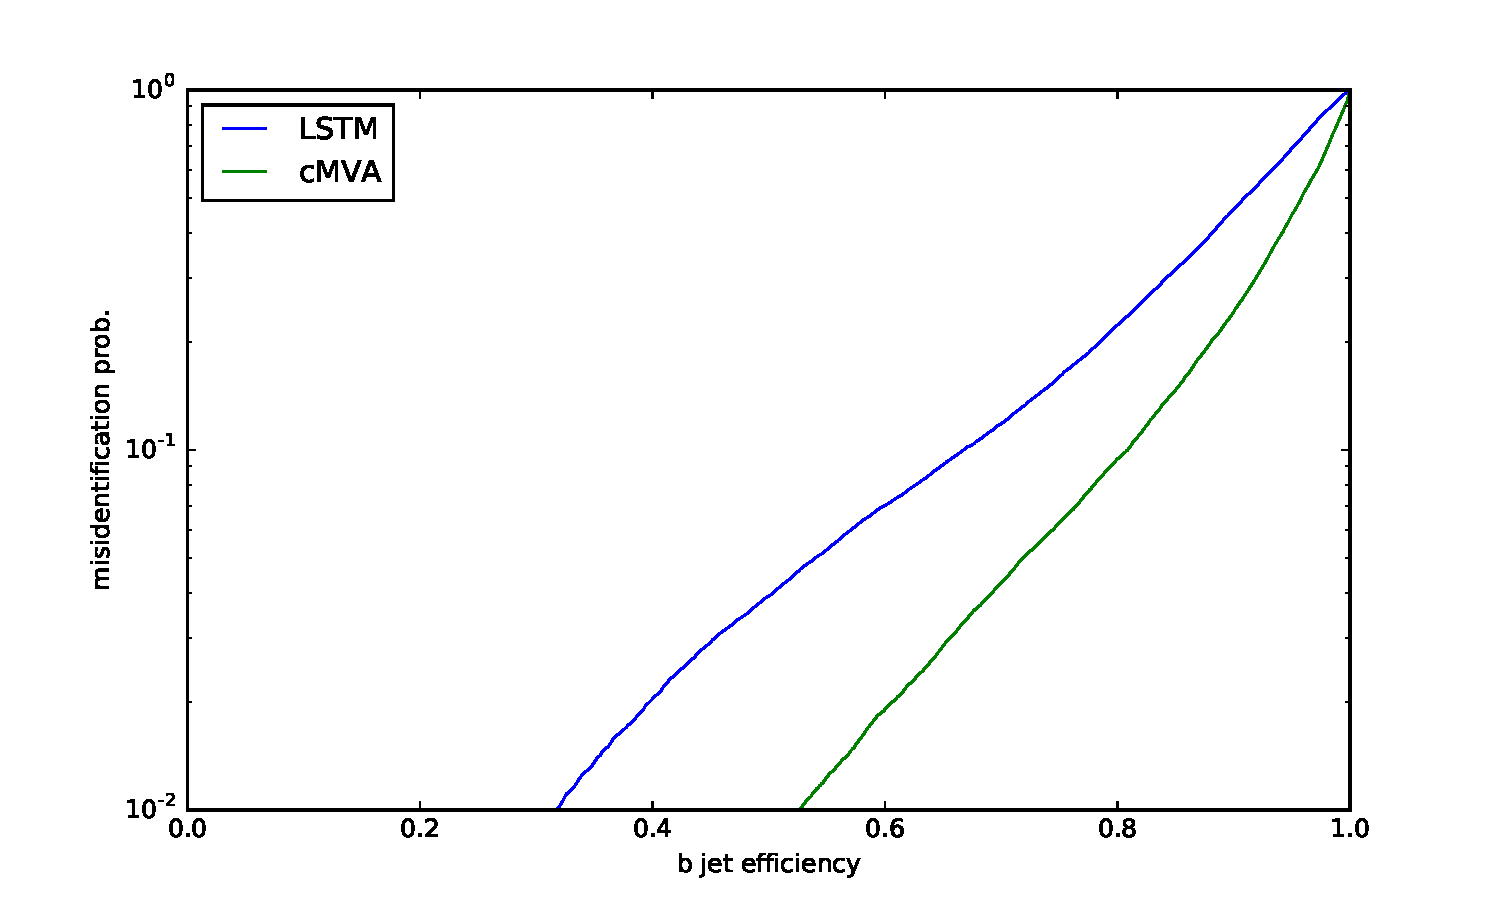
\includegraphics[width =0.5\textwidth]{../RNN_out/lstm64_3layers_singlestep_250_2/ROC-plot.pdf}\label{b}}

    \caption{ROC after 250 (left) and 500 training epochs (right) in comparison with the cMVA tagger.}
  \end{figure}

  Area under curve:
  \begin{itemize}
  \item AUC(cMVA) = 0.9233
  \item AUC(LSTM) = 0.8704
  \end{itemize}
  
\end{frame}


\begin{frame}
  \frametitle{64 nodes / layer, 3 layers}
  \framesubtitle{A different training strategy}
  Use 40 training epochs per 10k chunk (35 chunks in total):

    \begin{figure}[htb]
    \centering
    \subfloat[][]{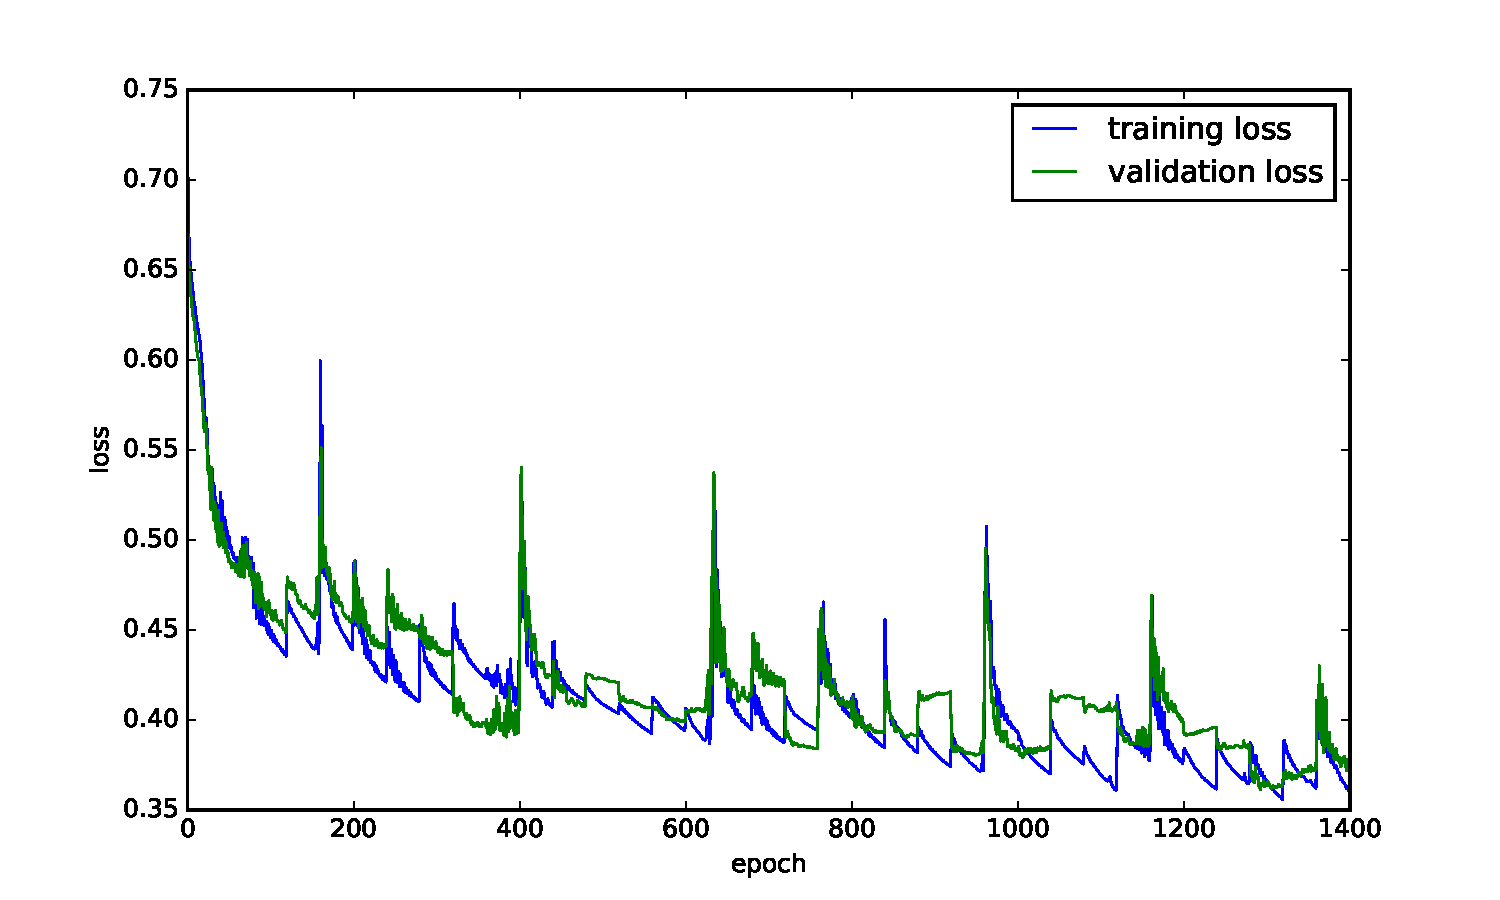
\includegraphics[width =0.5\textwidth]{../RNN_out/lstm64_3layers/loss-history.pdf}\label{a}}	
    \subfloat[][]{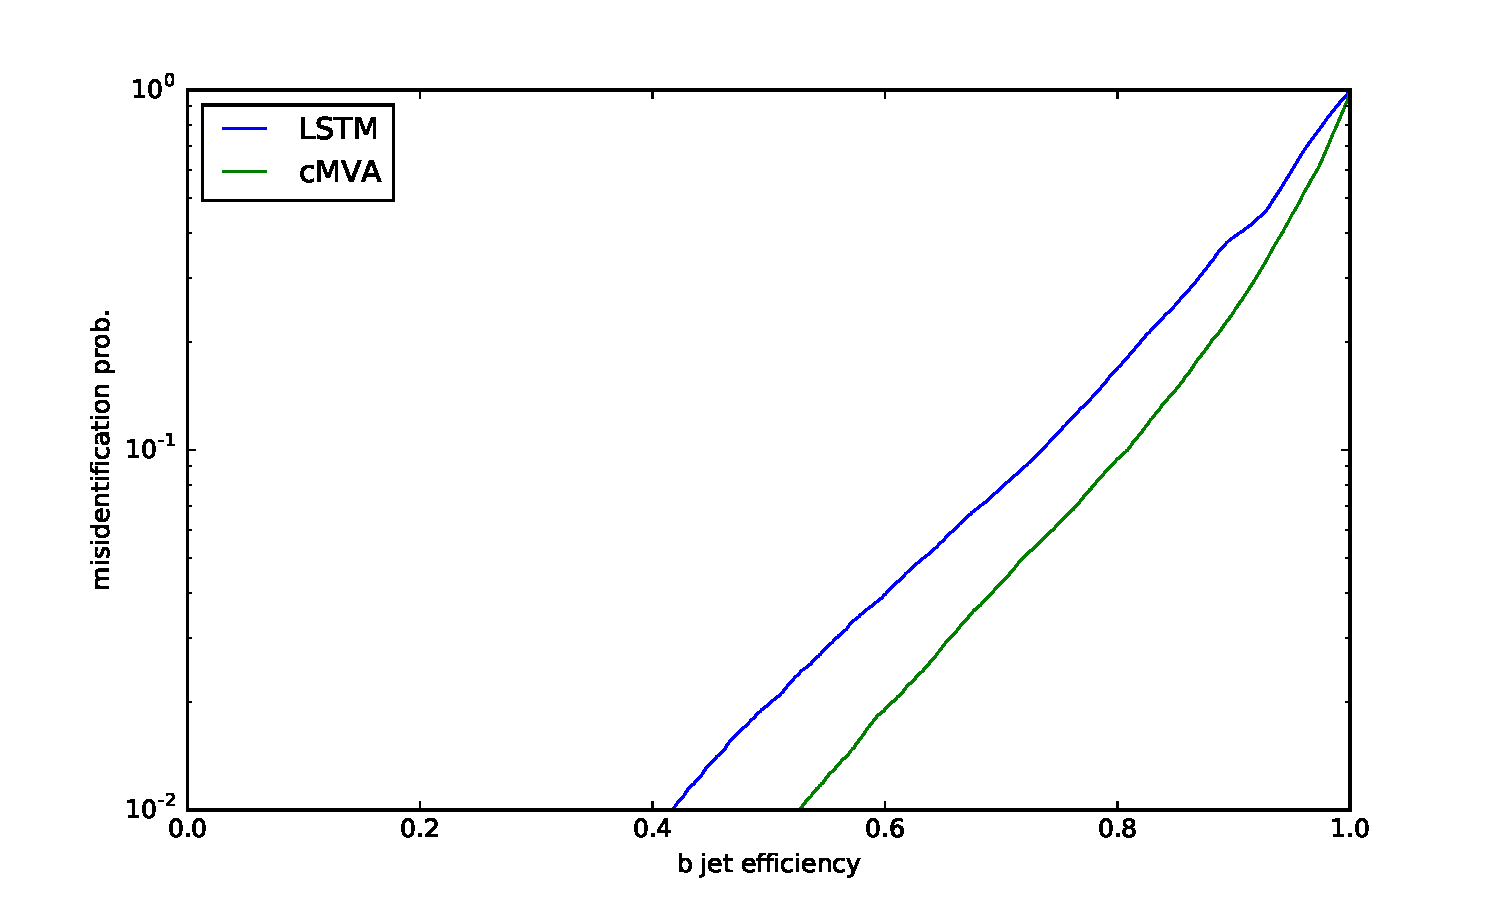
\includegraphics[width =0.5\textwidth]{../RNN_out/lstm64_3layers/ROC-plot-permanent.pdf}\label{b}}

    \caption{Loss function evolution (left) and ROC plot after completed training (right).}
    \end{figure}

    Area under curve:
    \begin{itemize}
    \item AUC(cMVA) = 0.9233
    \item AUC(LSTM) = 0.888
    \end{itemize}
\end{frame}

\begin{frame}
  \frametitle{64 nodes / layer, 3 layers}
  \framesubtitle{Output compared to cMVA, modified training strategy}
  \begin{figure}[htb]
    \centering
    \subfloat[][]{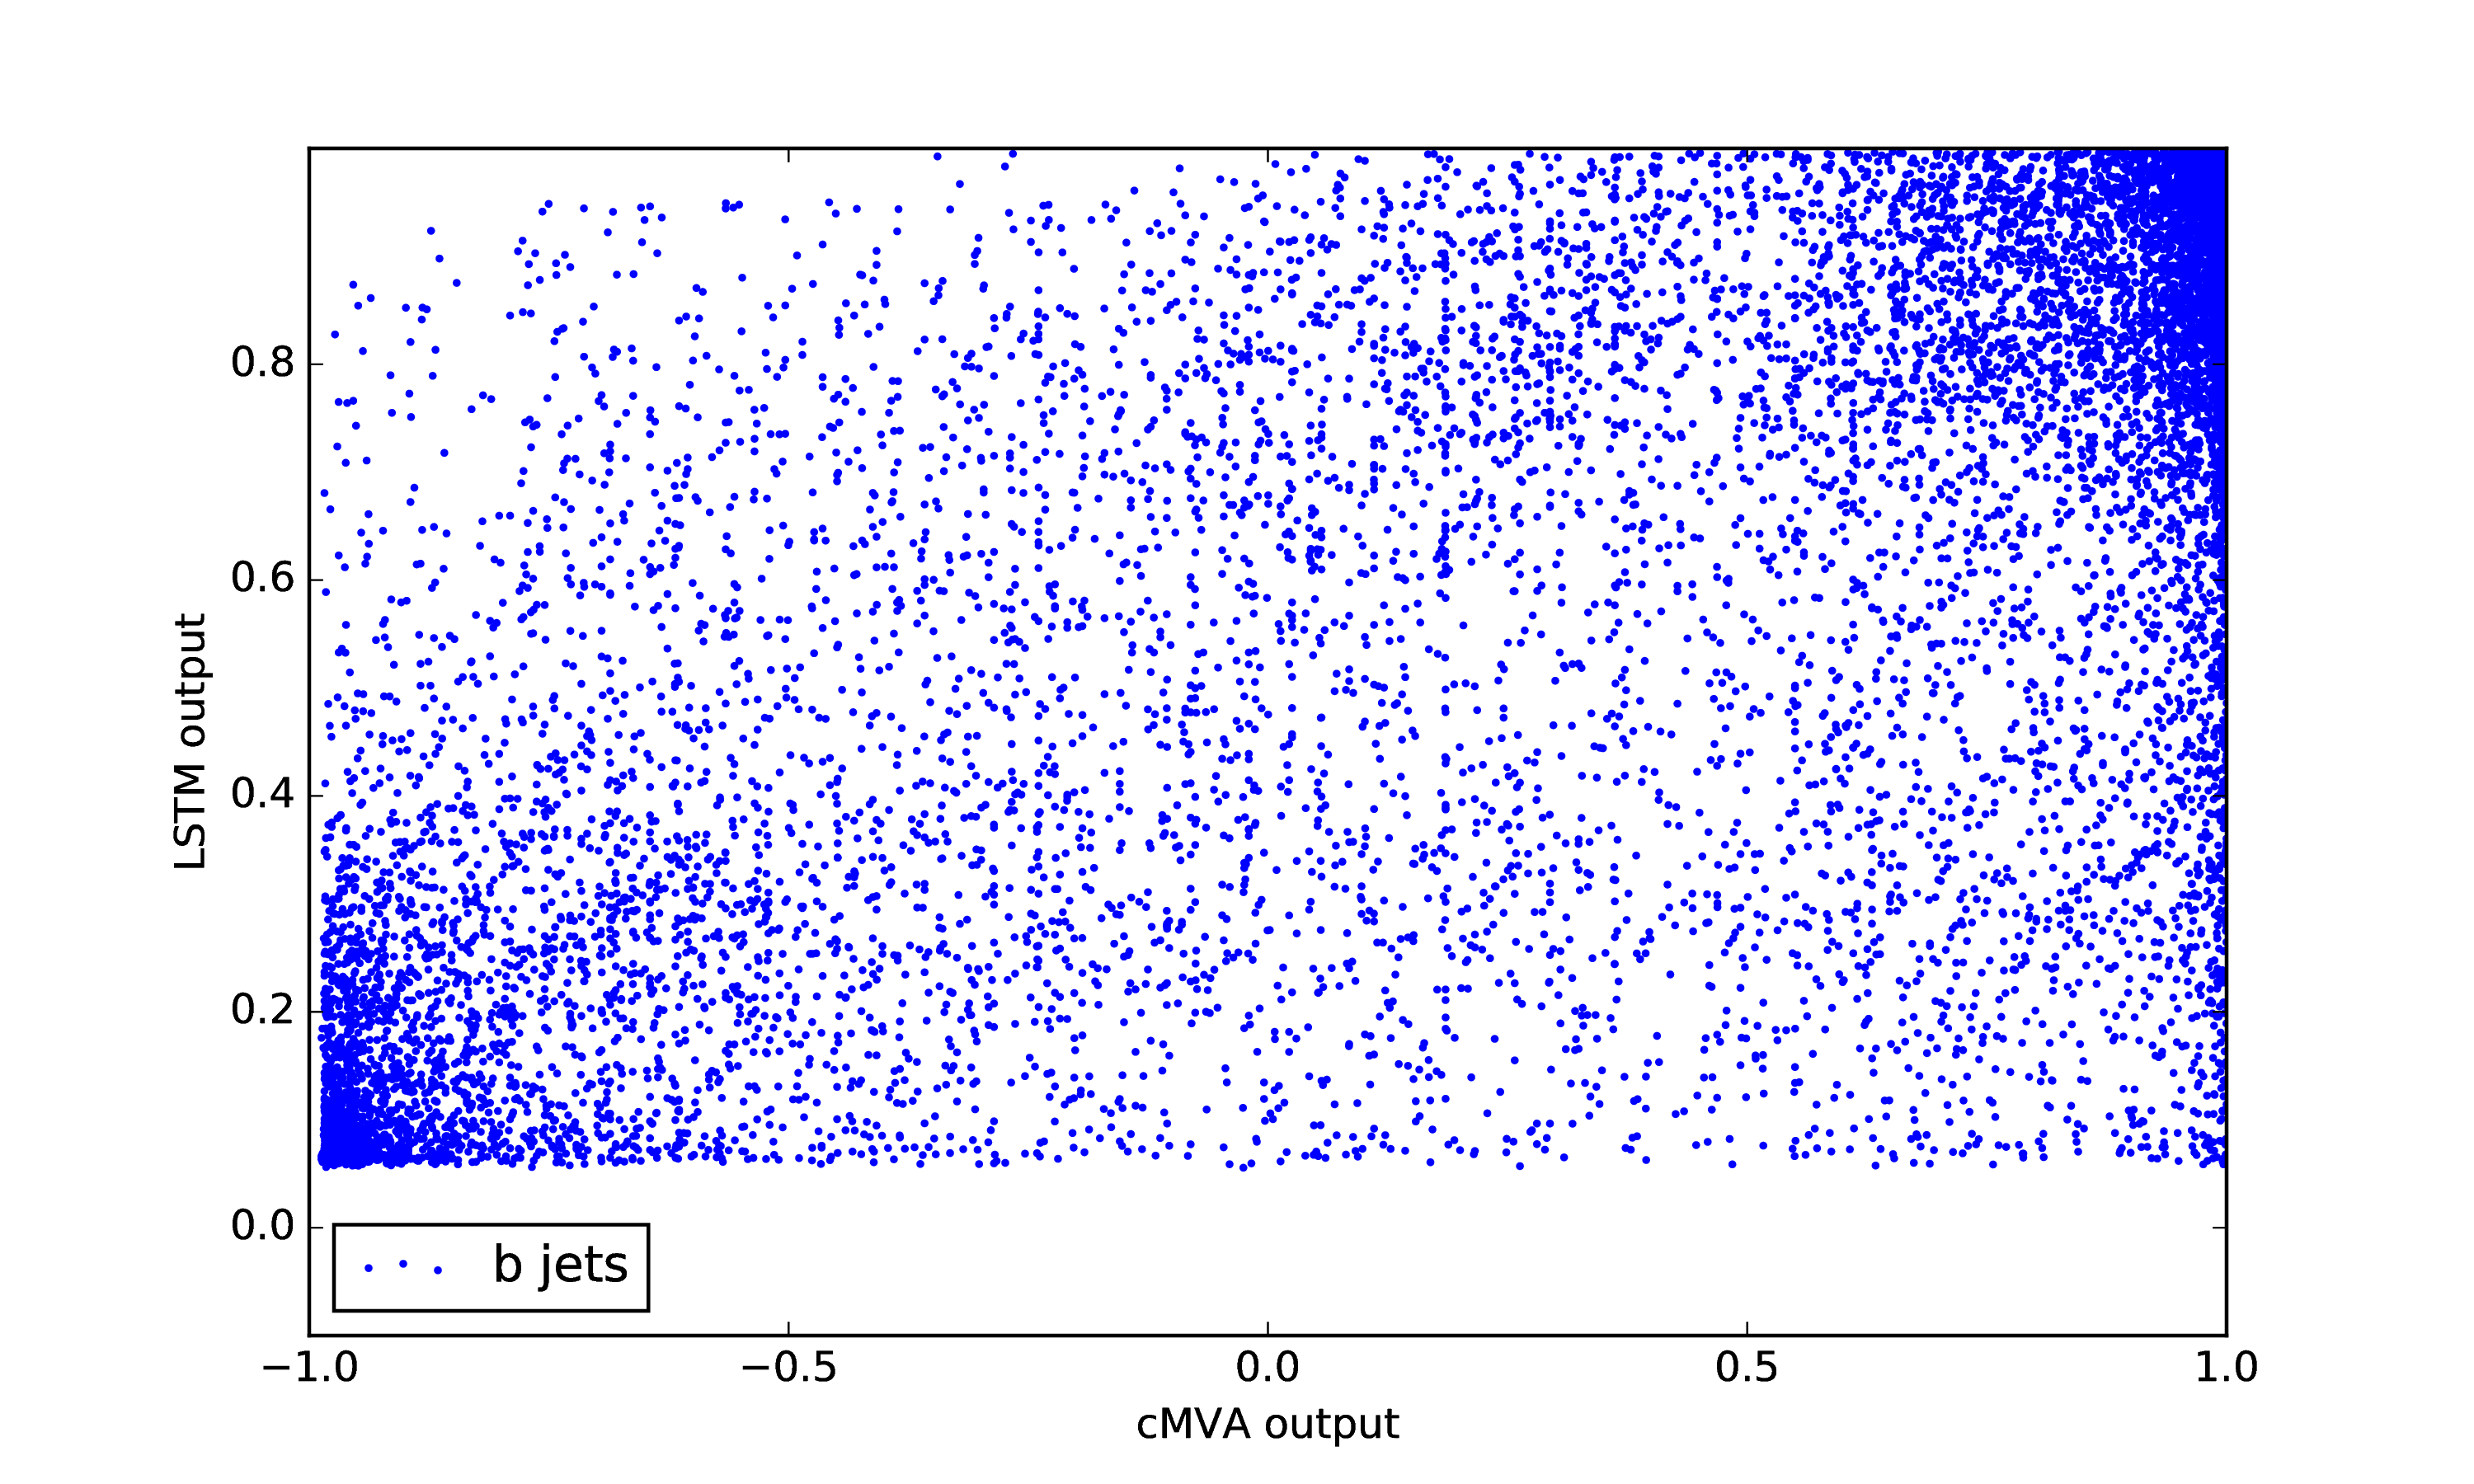
\includegraphics[width =0.5\textwidth]{../RNN_out/lstm64_3layers/ROC-scatter-signal.png}\label{a}}	
    \subfloat[][]{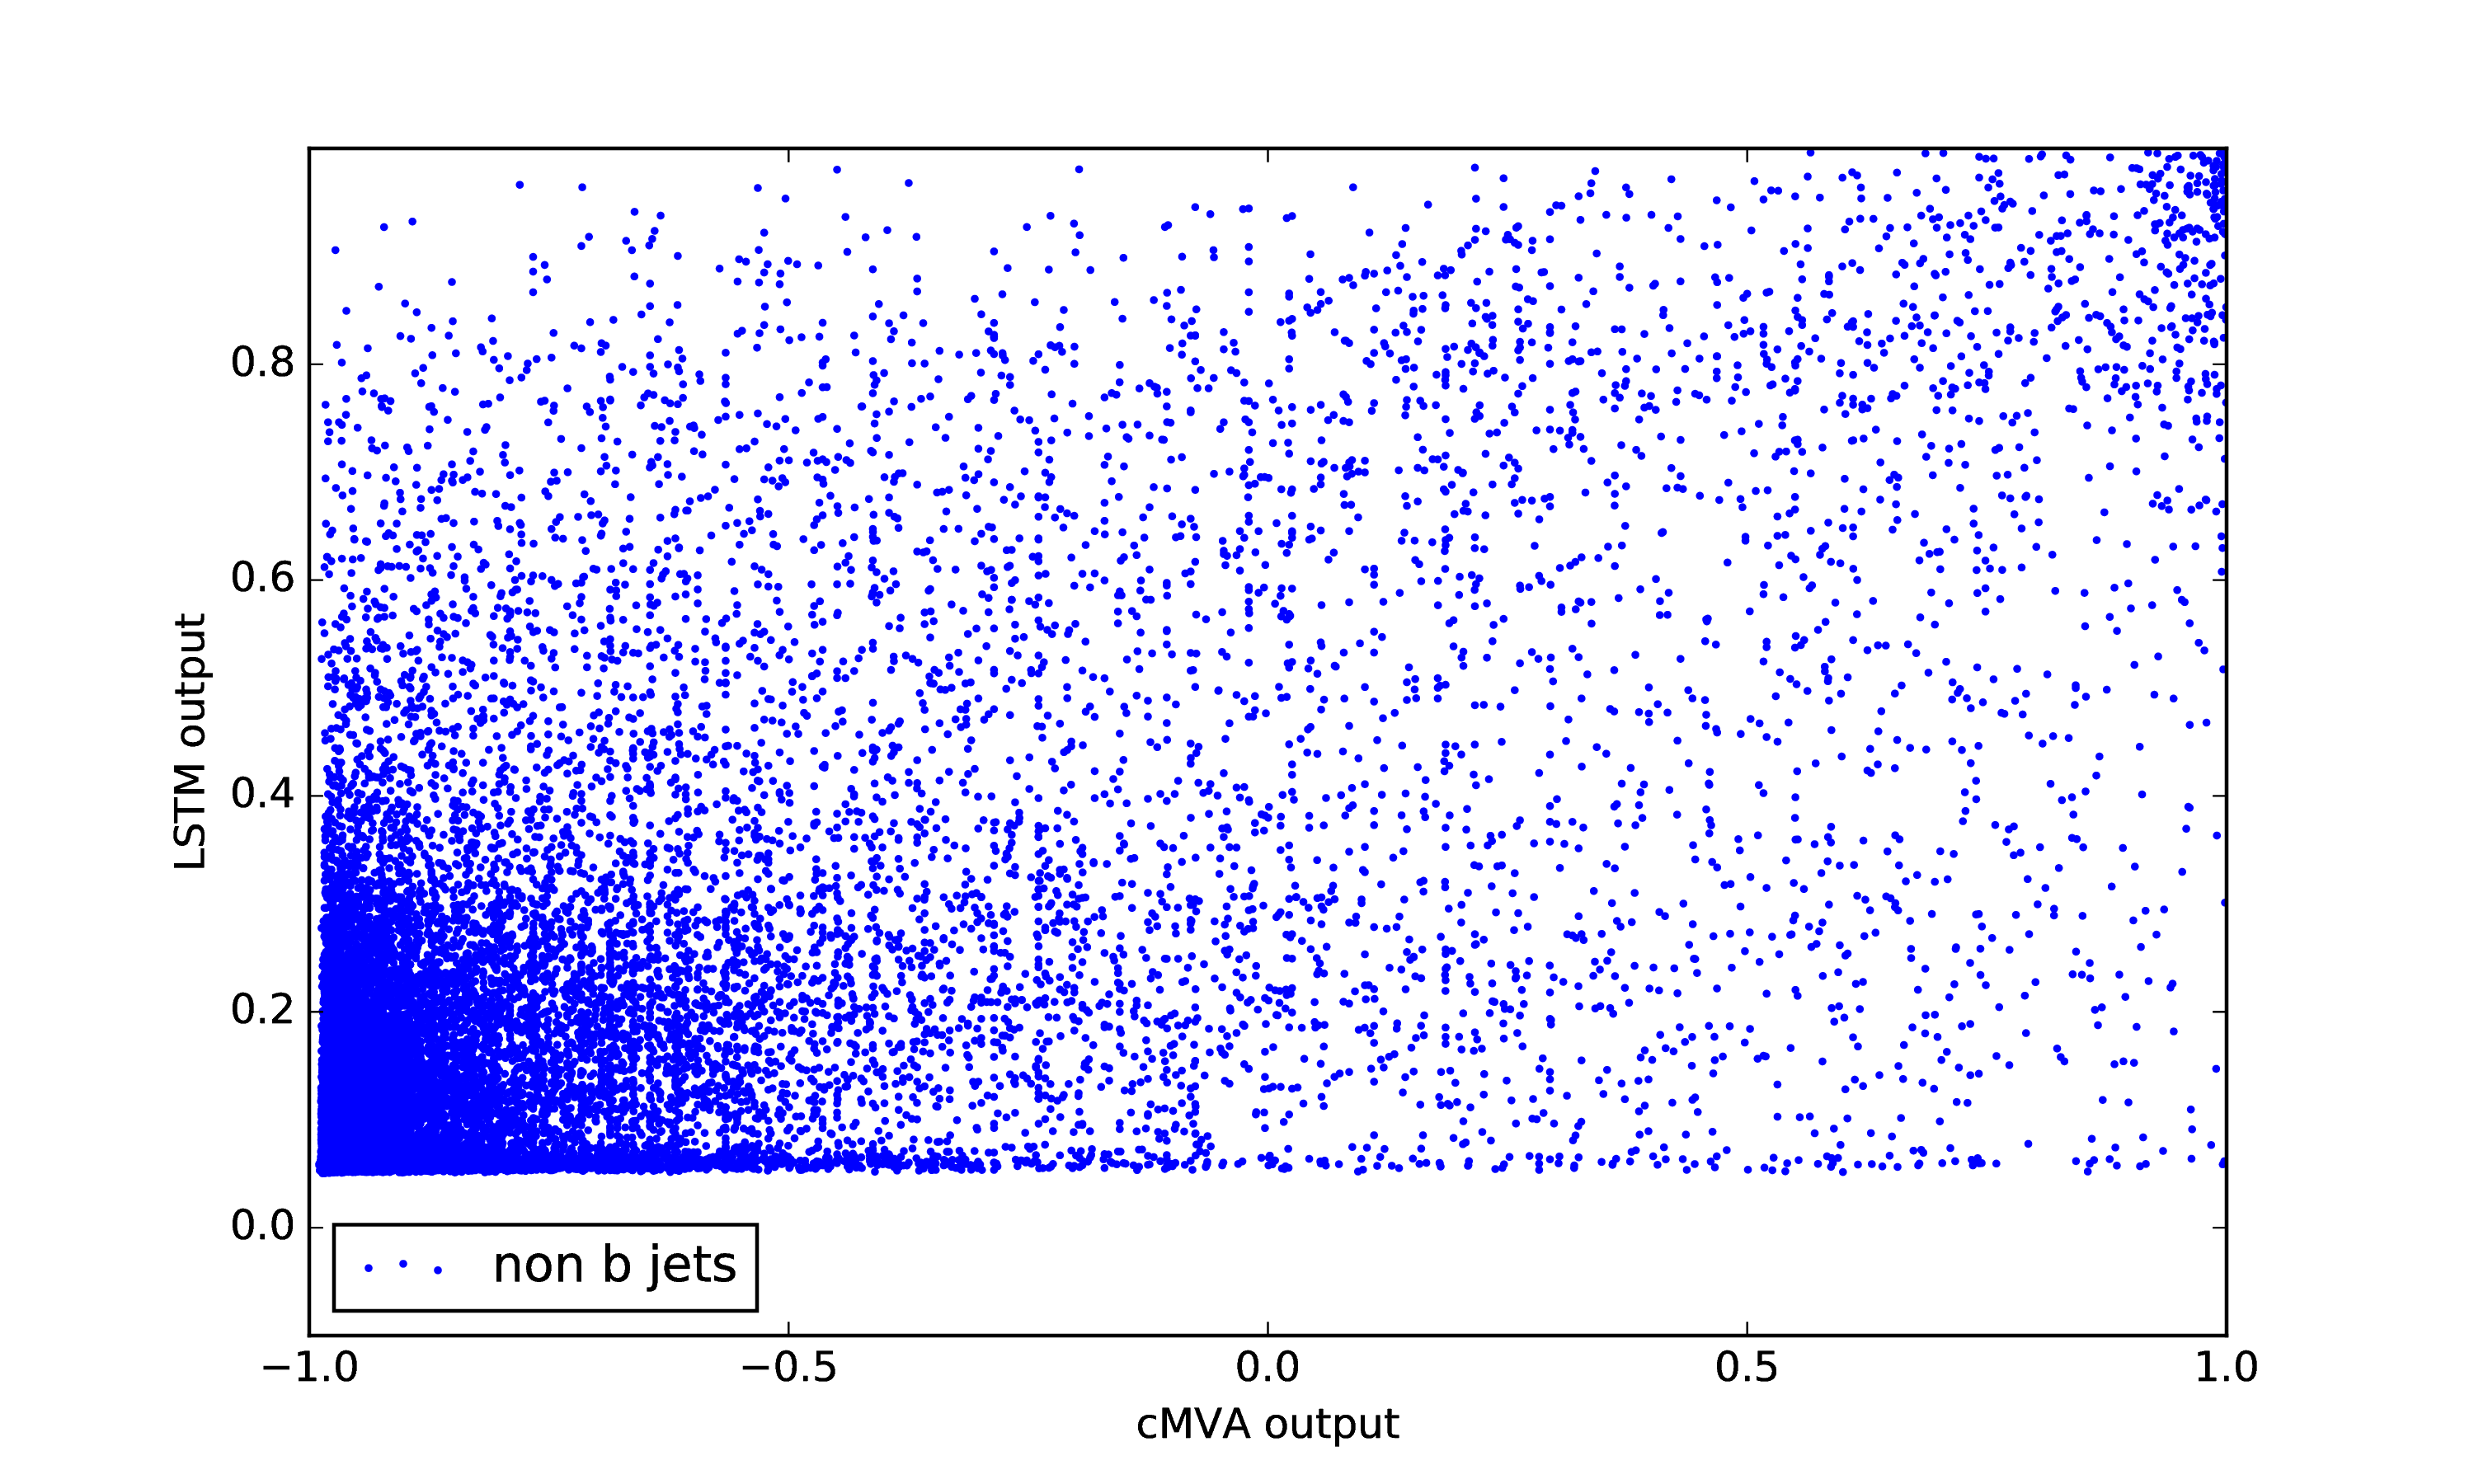
\includegraphics[width =0.5\textwidth]{../RNN_out/lstm64_3layers/ROC-scatter-background.png}\label{b}}

    \caption{Output of the LSTM tagger in comparison with the cMVA output: signal events shown left, background right.}
  \end{figure}
\end{frame}


\begin{frame}
  \frametitle{128 nodes / layer, 1 layer}

  \begin{figure}[htb]
    \centering
    \subfloat[][]{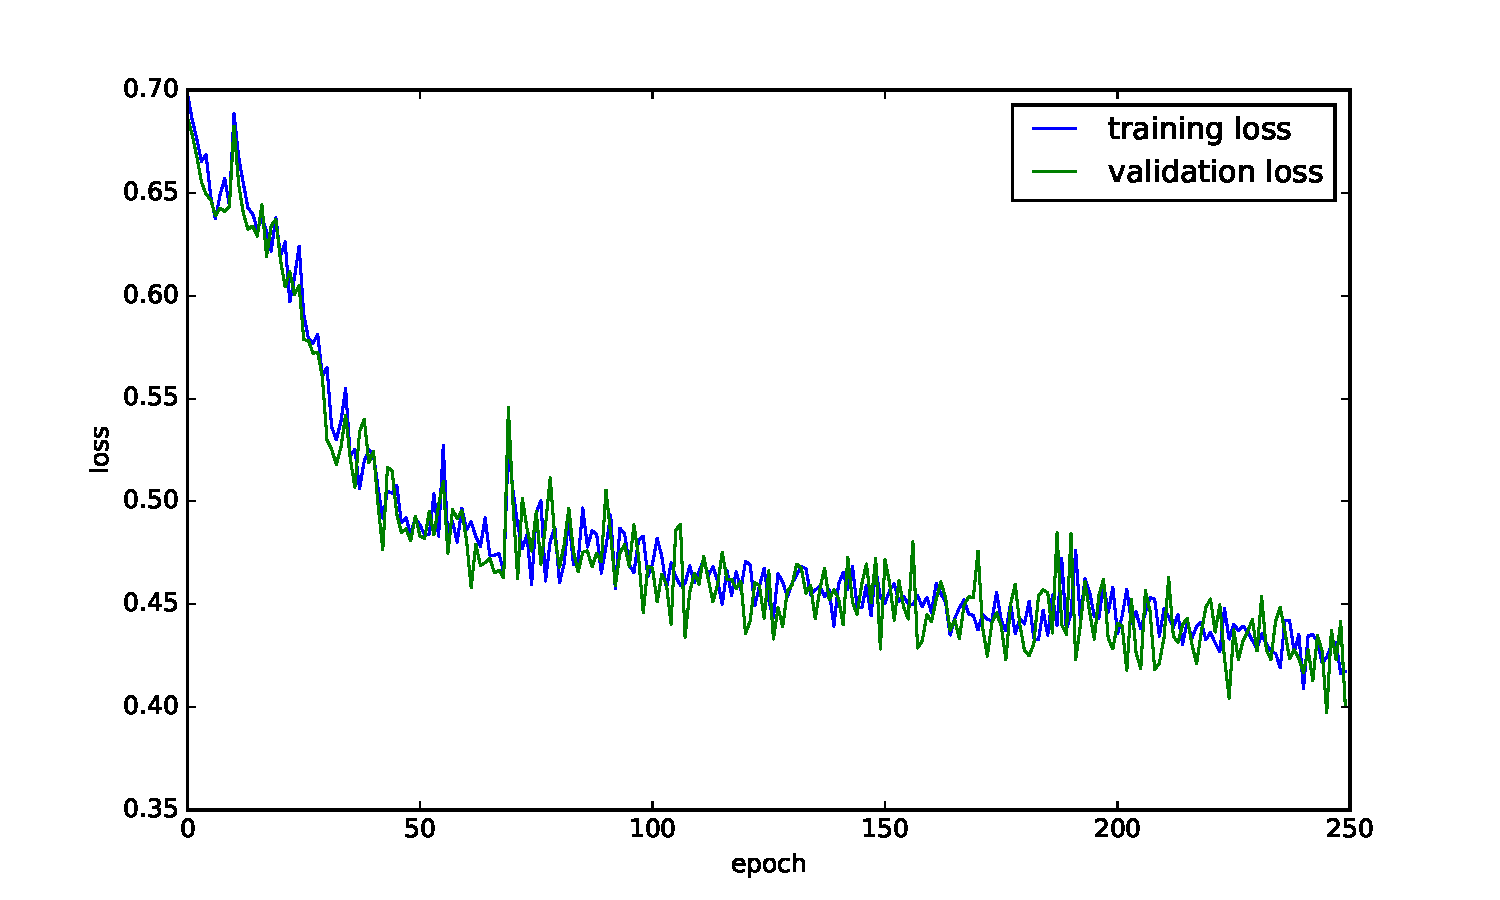
\includegraphics[width =0.5\textwidth]{../RNN_out/lstm128_1layer_singlestep_250/loss-history.pdf}\label{a}}	
    \subfloat[][]{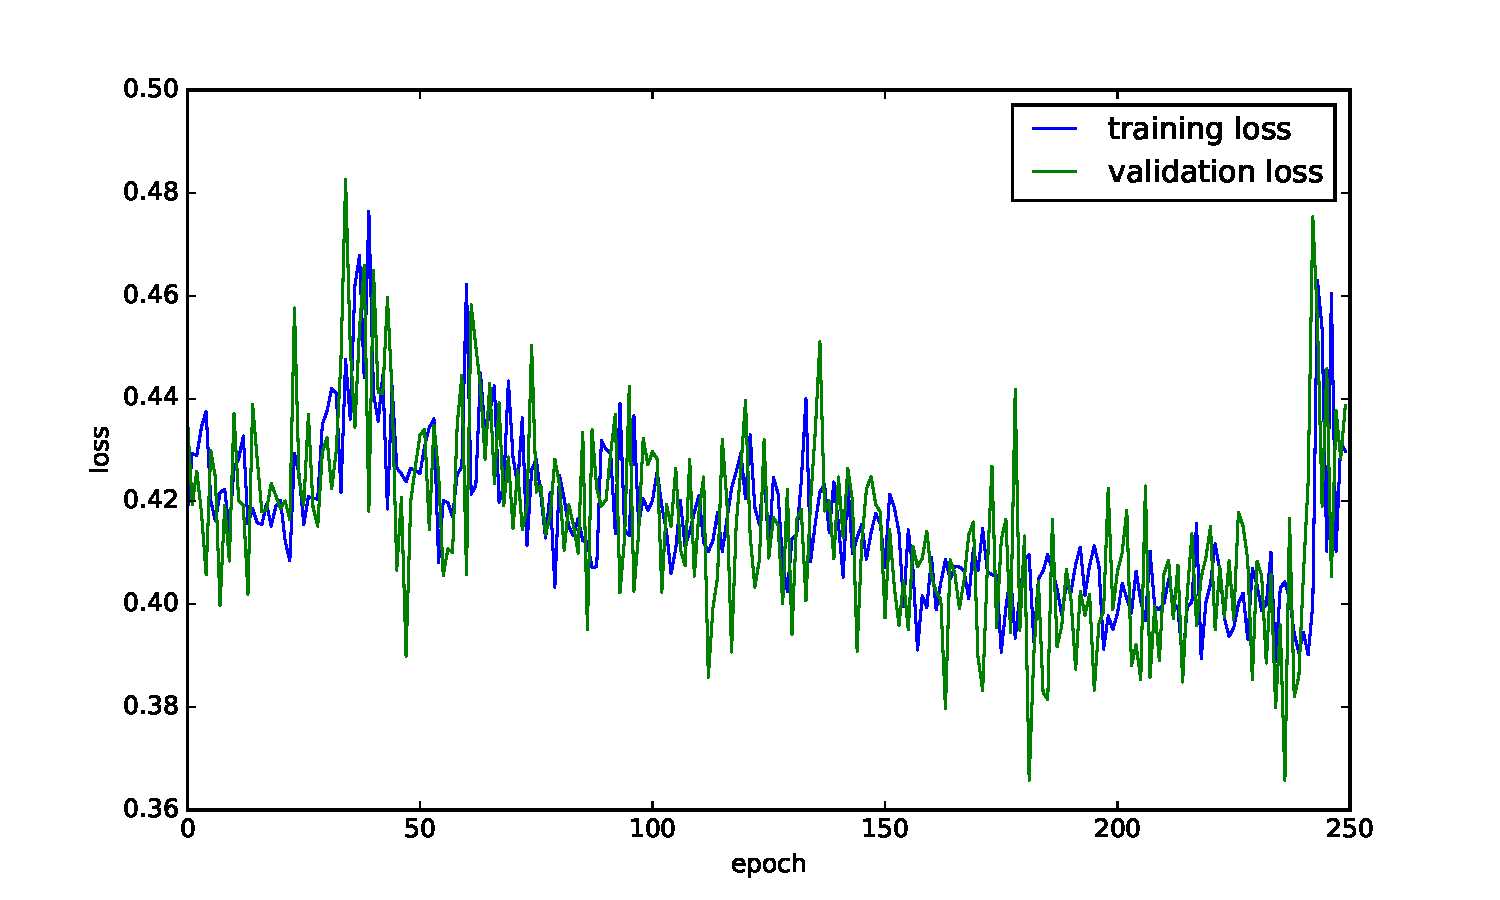
\includegraphics[width =0.5\textwidth]{../RNN_out/lstm128_1layer_singlestep_250_2/loss-history.pdf}\label{b}}

    \caption{Loss function (binary cross-entropy) for epochs 1-250 (left) and 250-500 (right).}
  \end{figure}

\end{frame}


\begin{frame}
  \frametitle{128 nodes / layer, 1 layer}

  \begin{figure}[htb]
    \centering
    \subfloat[][]{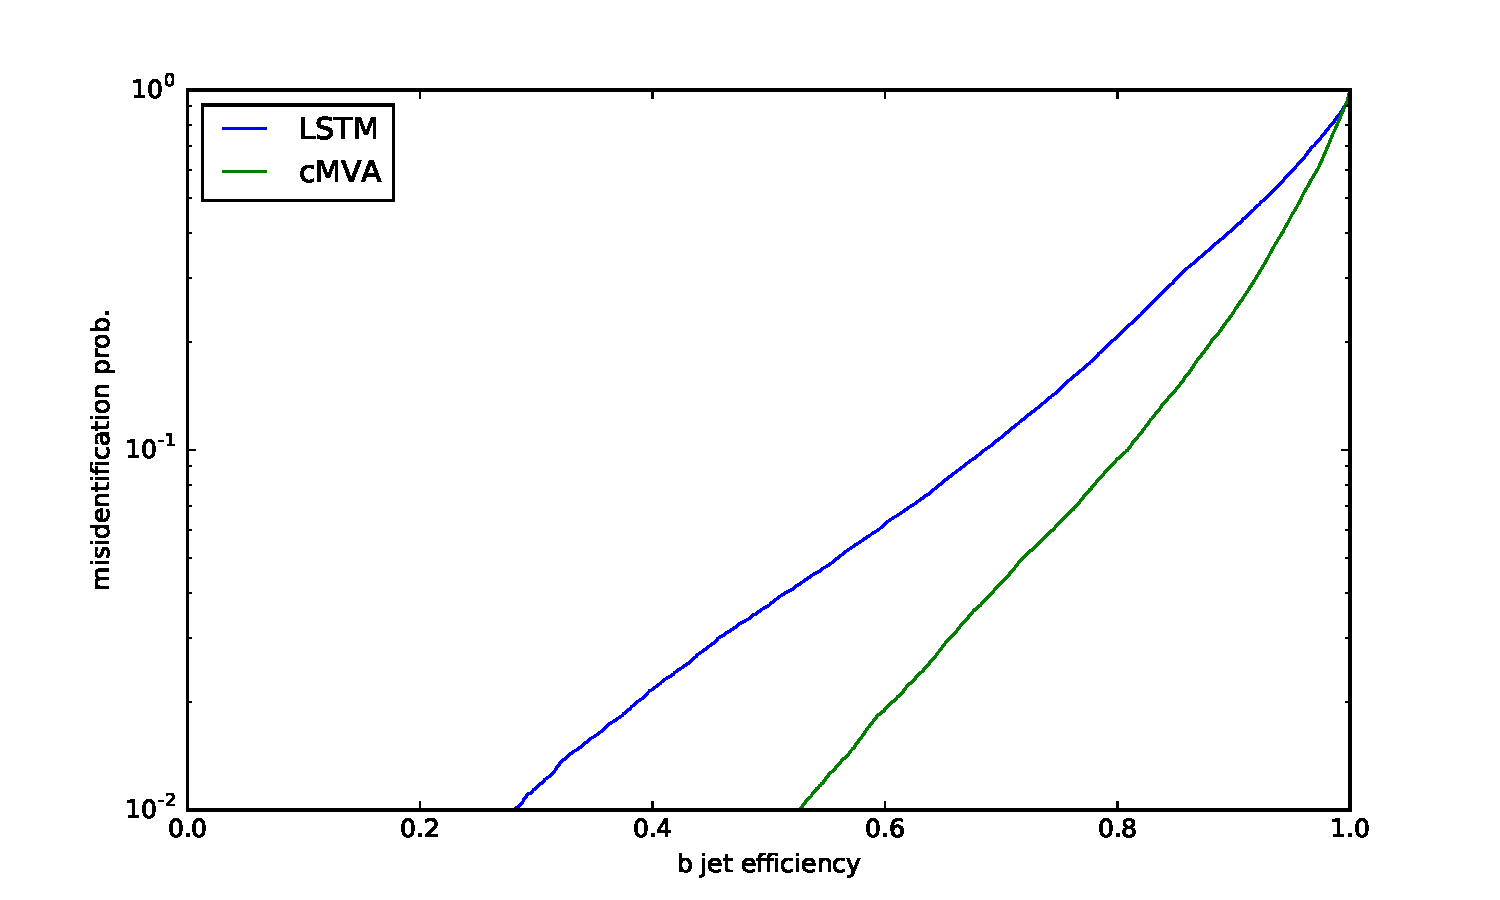
\includegraphics[width =0.5\textwidth]{../RNN_out/lstm128_1layer_singlestep_250/ROC-plot.pdf}\label{a}}	
    \subfloat[][]{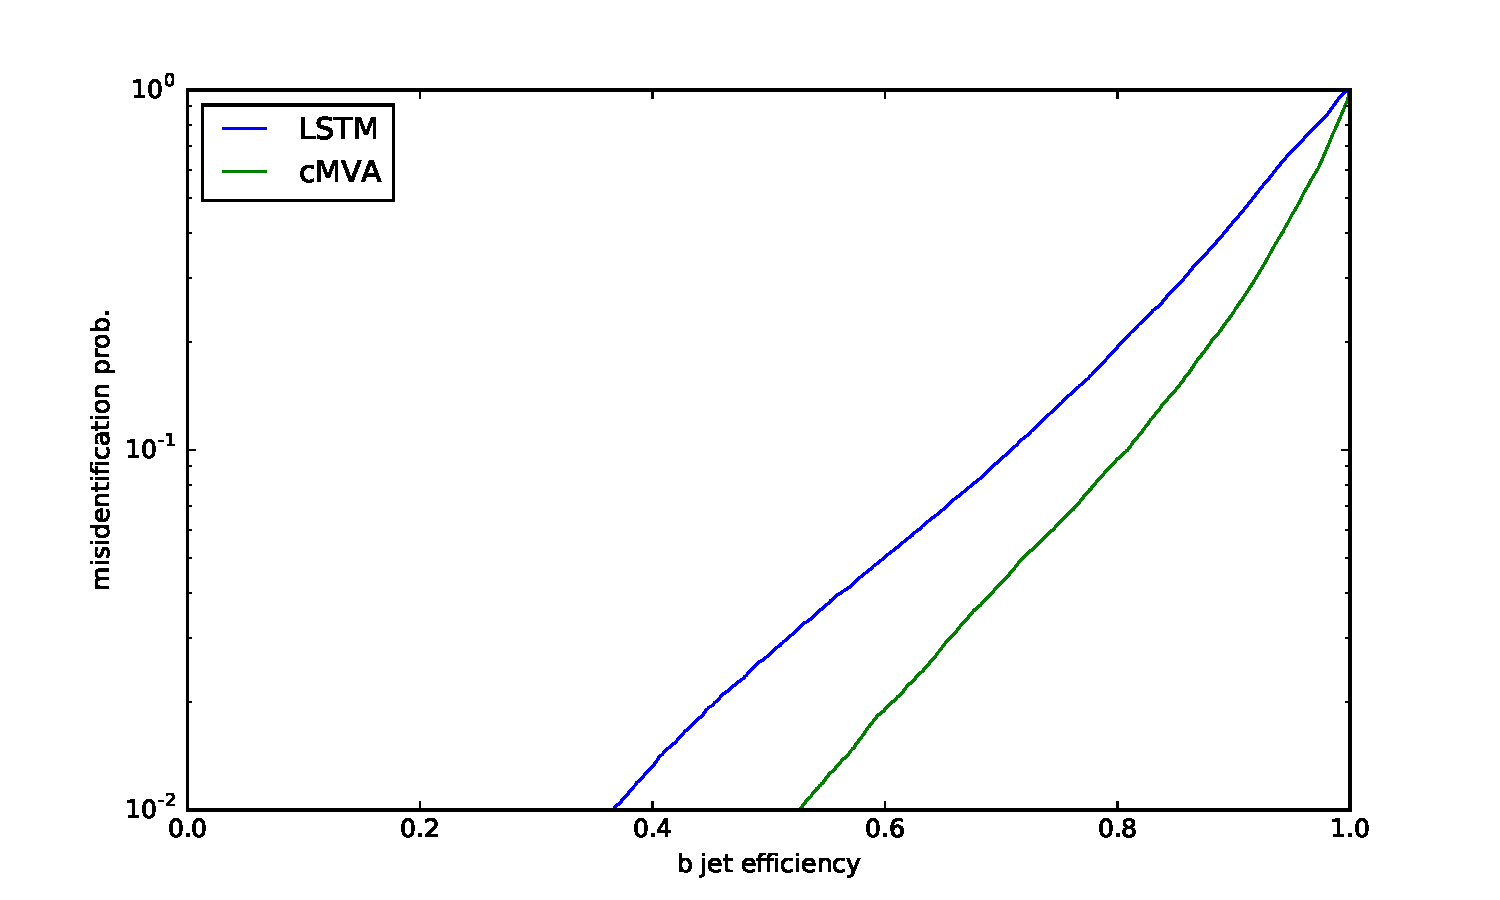
\includegraphics[width =0.5\textwidth]{../RNN_out/lstm128_1layer_singlestep_250_2/ROC-plot-permanent.pdf}\label{b}}

    \caption{ROC after 250 (left) and 500 training epochs (right) in comparison with the cMVA tagger.}
  \end{figure}

  \begin{itemize}
  \item AUC(cMVA) = 0.9233
  \item AUC(LSTM) = 0.8737
  \end{itemize}

\end{frame}

\begin{frame}
  \frametitle{128 nodes / layer, 1 layer}
  \framesubtitle{Output compared to cMVA}
  \begin{figure}[htb]
    \centering
    \subfloat[][]{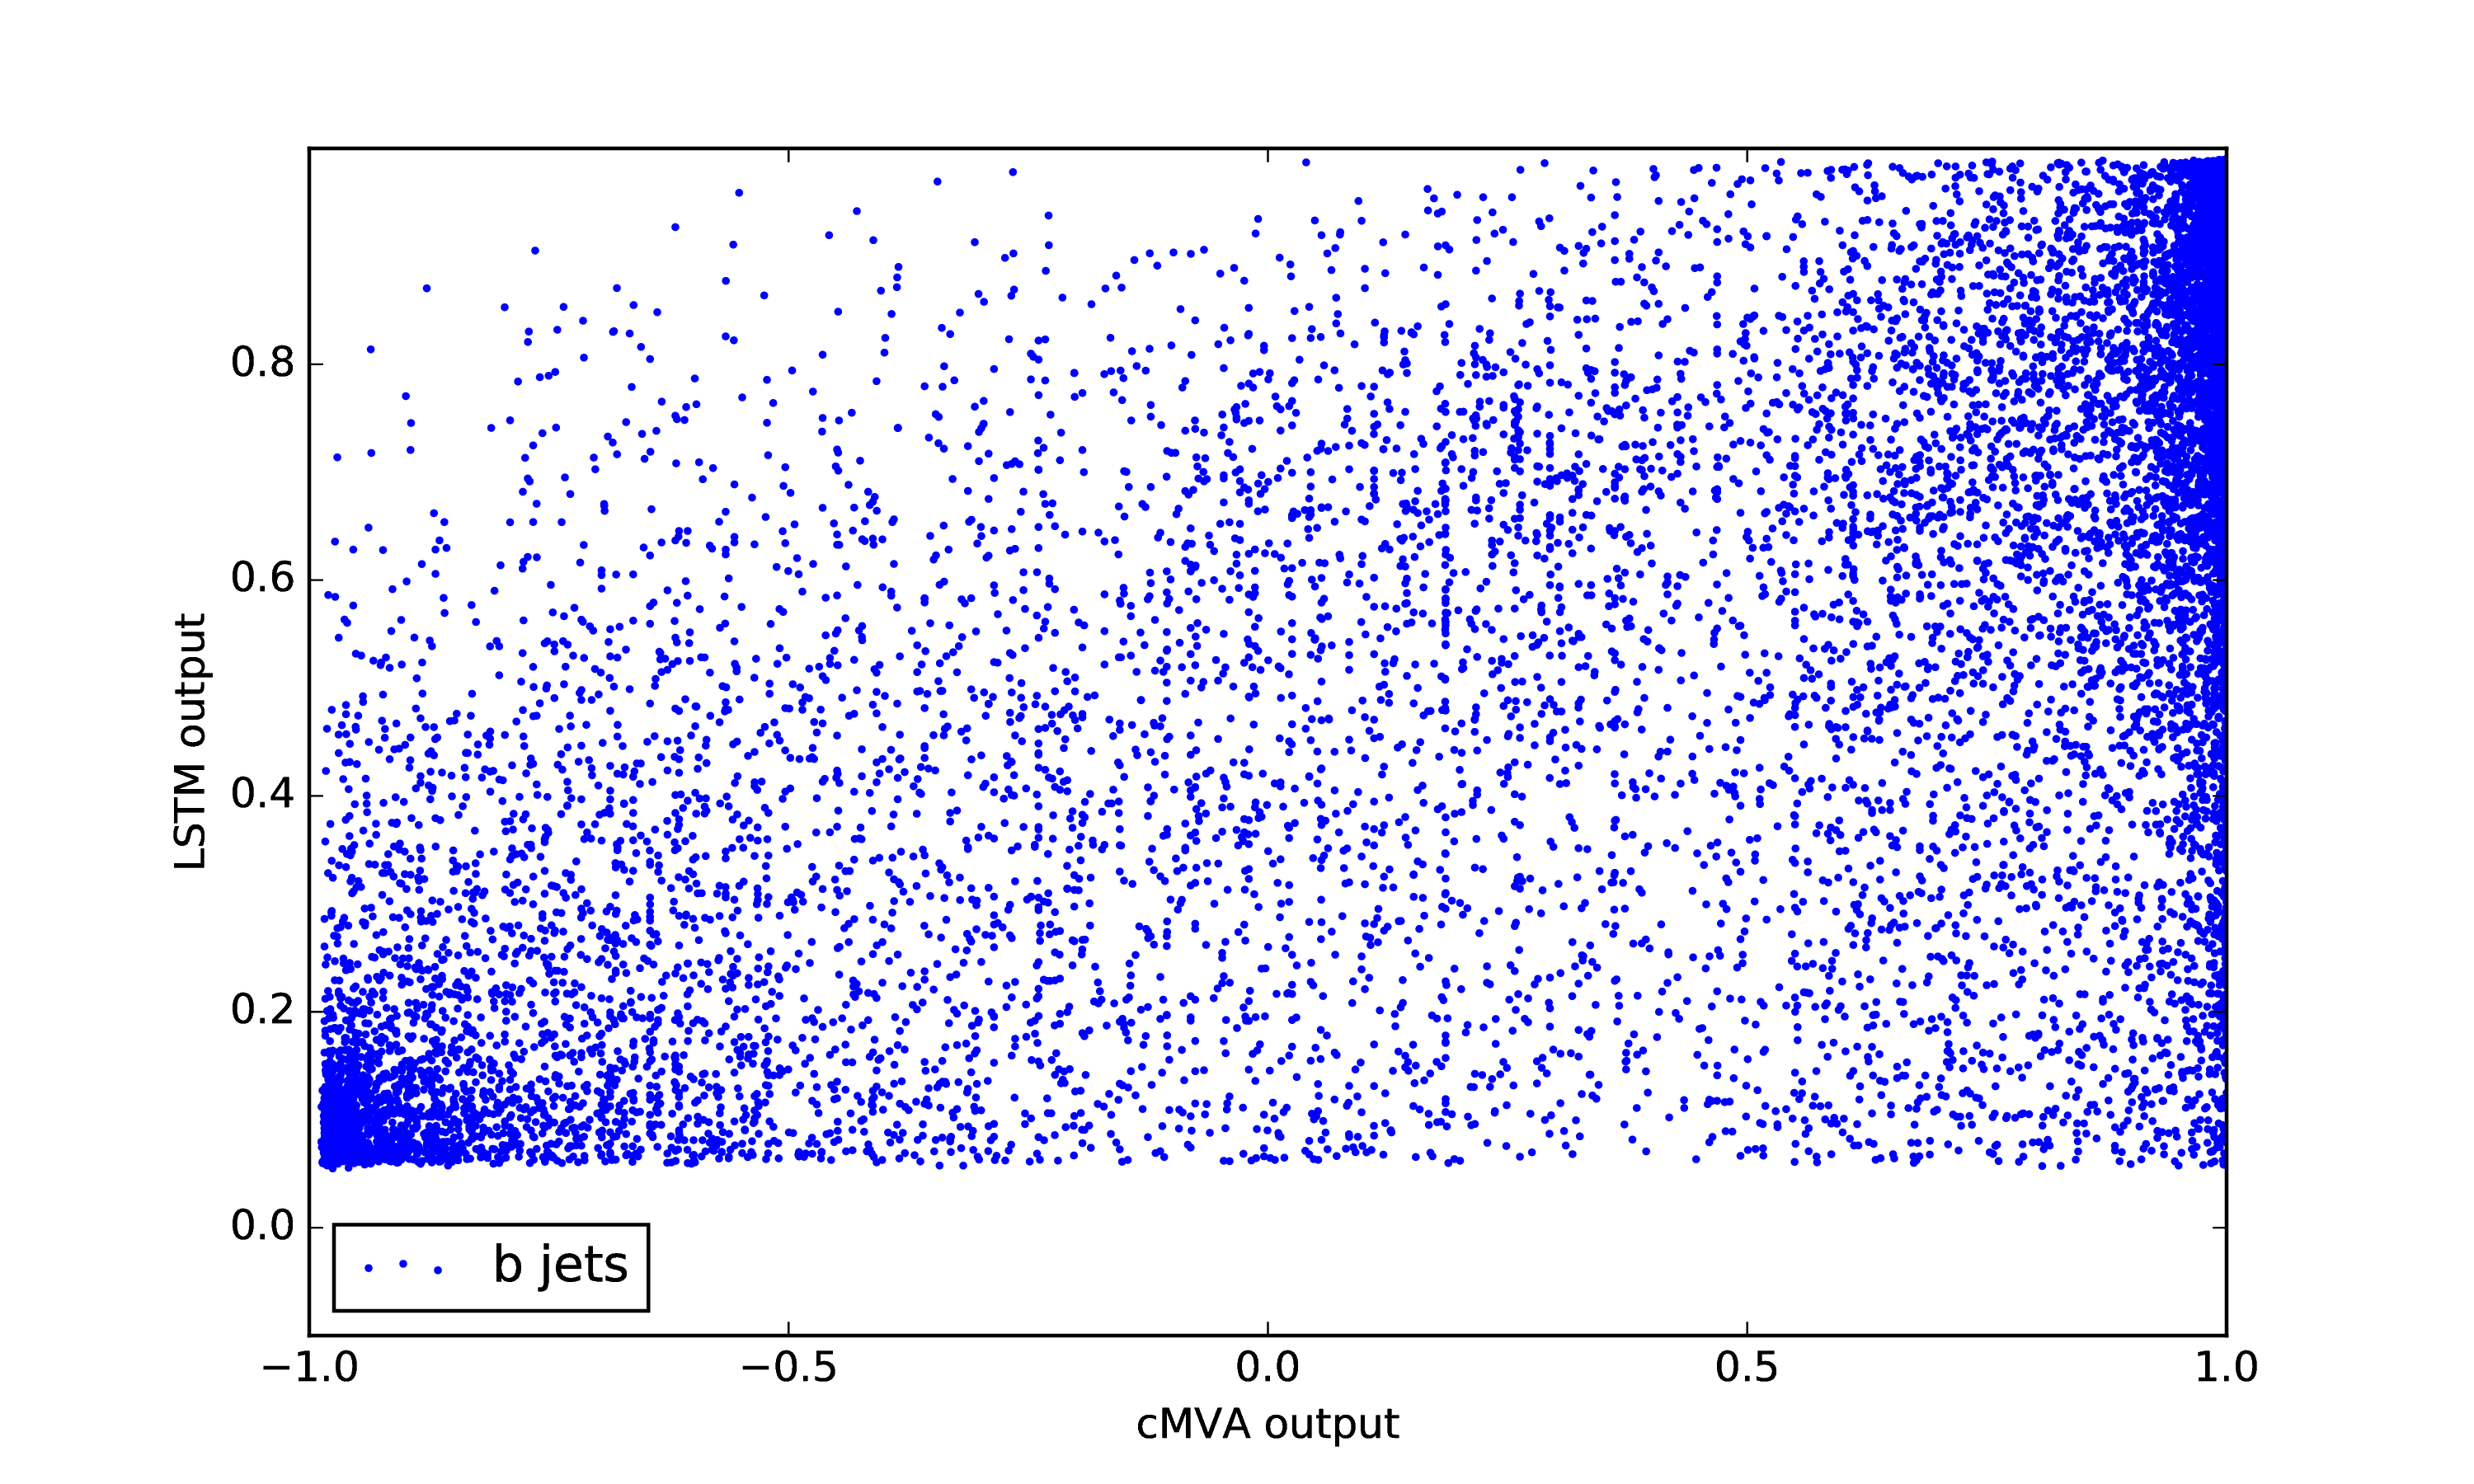
\includegraphics[width =0.5\textwidth]{../RNN_out/lstm128_1layer_singlestep_250_2/ROC-scatter-signal.png}\label{a}}	
    \subfloat[][]{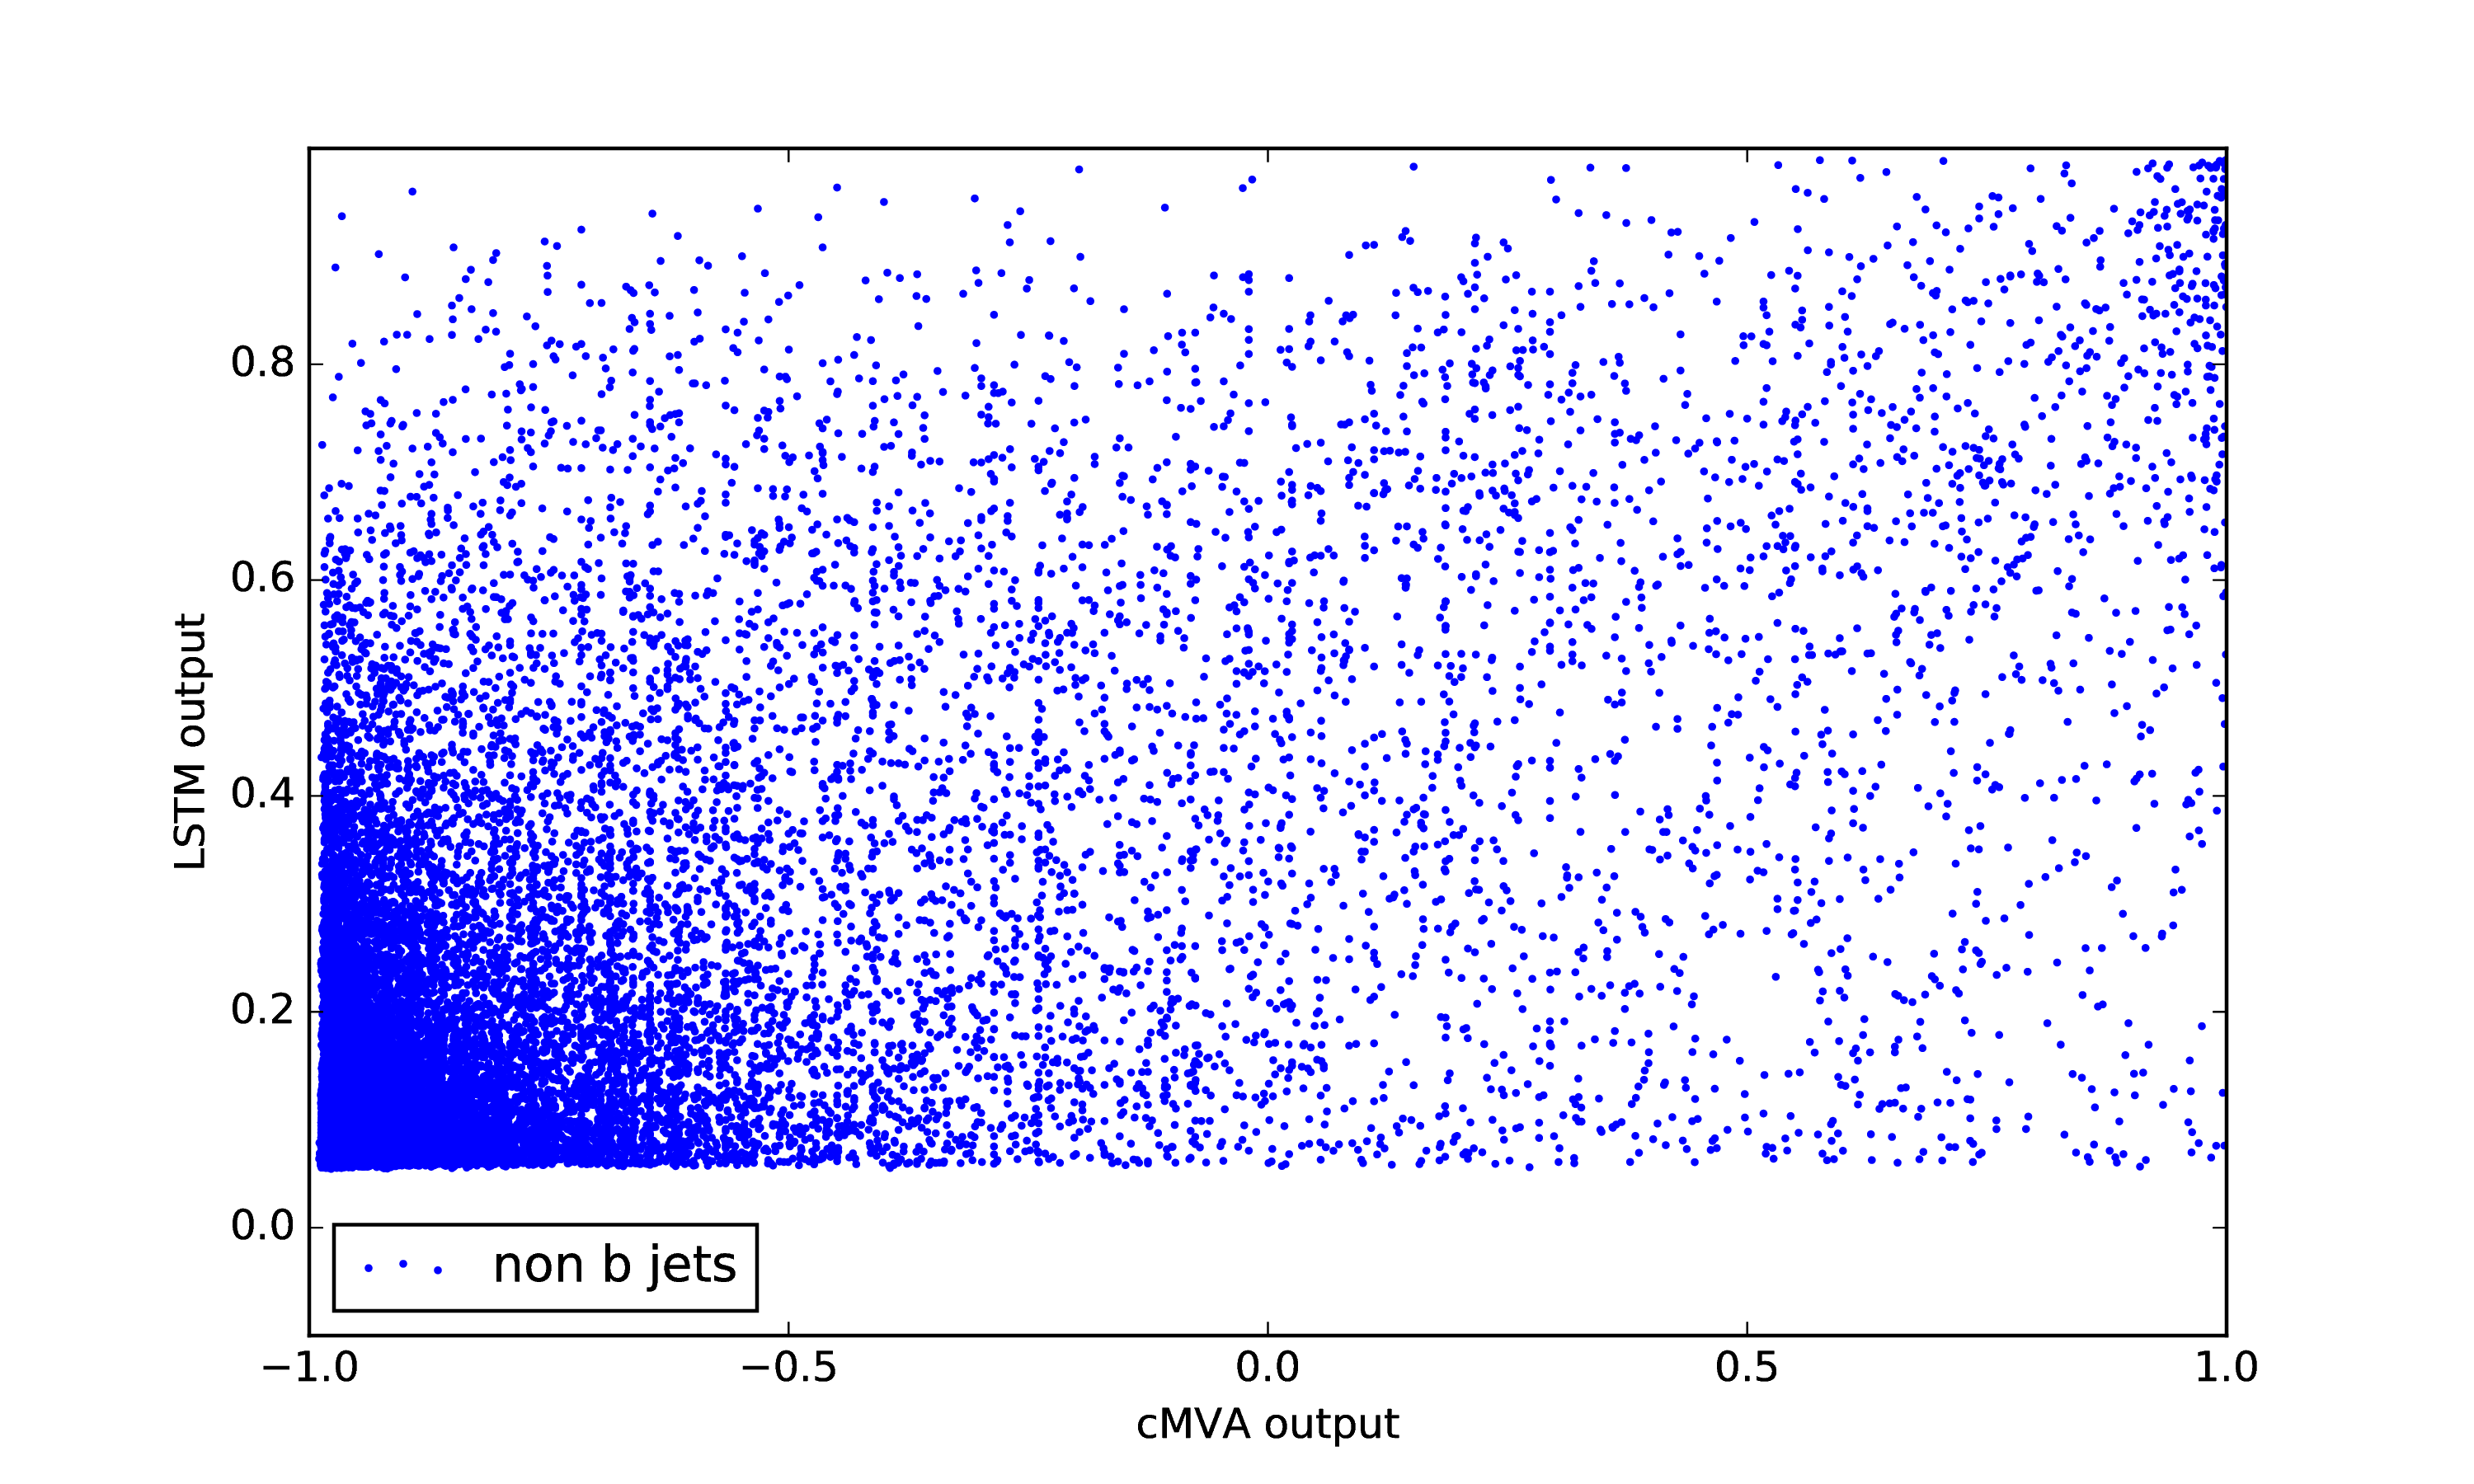
\includegraphics[width =0.5\textwidth]{../RNN_out/lstm128_1layer_singlestep_250_2/ROC-scatter-background.png}\label{b}}

    \caption{Output of the LSTM tagger in comparison with the cMVA output: signal events shown left, background right.}
  \end{figure}
\end{frame}

\begin{frame}
  \frametitle{LSTM64 / 3: Training with reduced track parameters}
  \framesubtitle{Reference run}
  Setup: 40 epochs per chunk, 50 chunks (each containing 10k jets)

  Use all track parameters for a reference run:
  \begin{figure}
    \centering
    \subfloat[][]{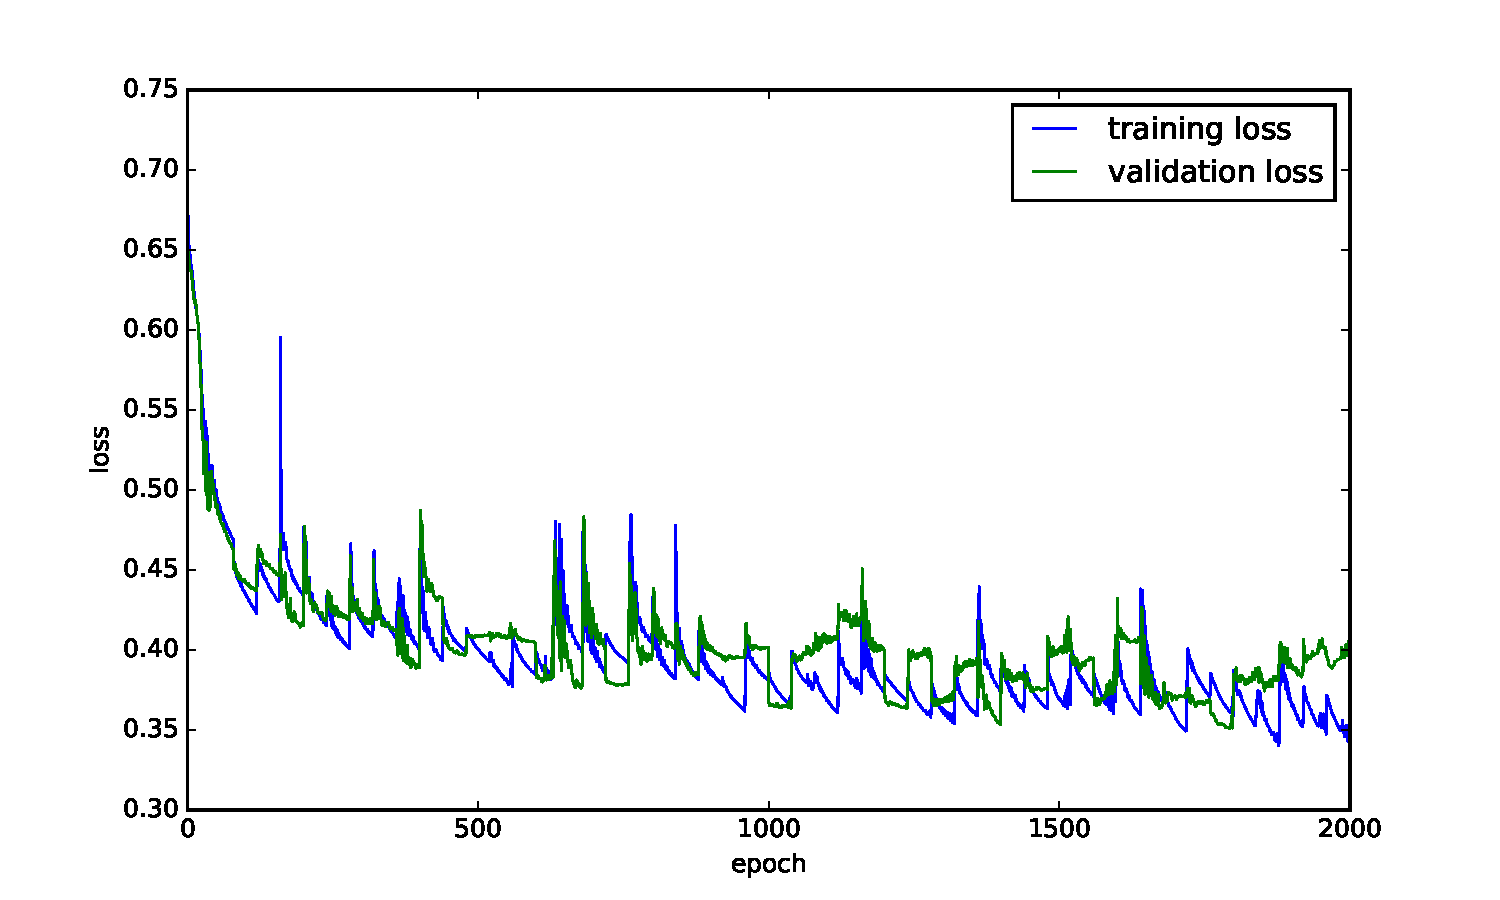
\includegraphics[width =0.5\textwidth]{../RNN_out/lstm64_3layers_allparams/loss-history.pdf}\label{a}}	
    \subfloat[][]{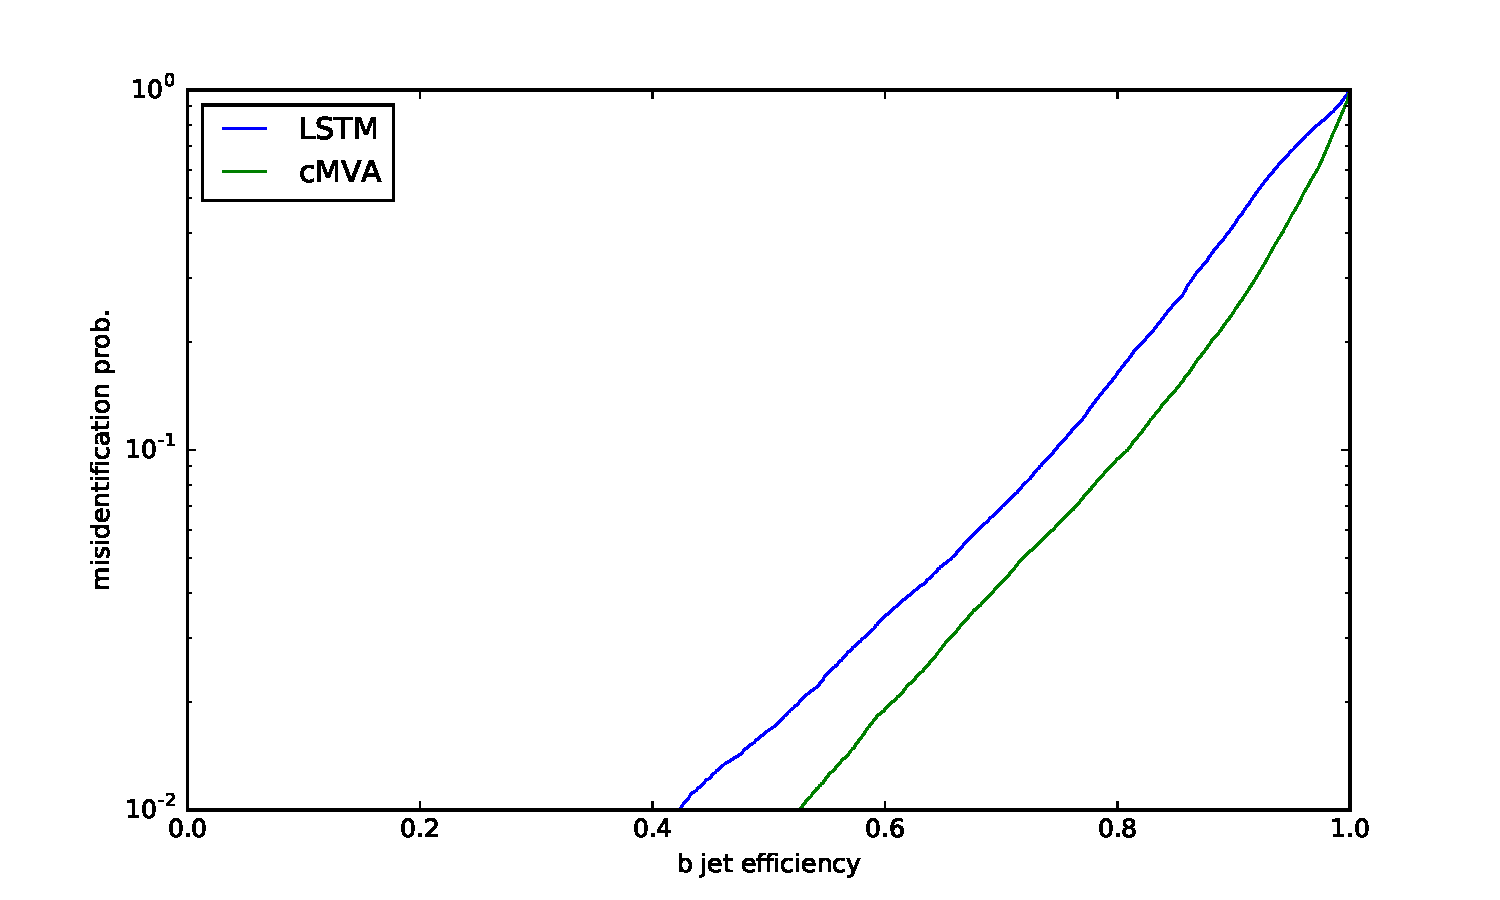
\includegraphics[width =0.5\textwidth]{../RNN_out/lstm64_3layers_allparams/ROC-plot.pdf}\label{b}}
  \end{figure}

  overtraining??
  
  \begin{itemize}
  \item AUC(cMVA) = 0.9233
  \item AUC(LSTM) = 0.8843
  \end{itemize}
\end{frame}

\begin{frame}
  \frametitle{LSTM64 / 3: Training with reduced track parameters}
  \framesubtitle{without \texttt{Track\_IP} and \texttt{Track\_IP2D}}

  \begin{figure}
    \centering
    \subfloat[][]{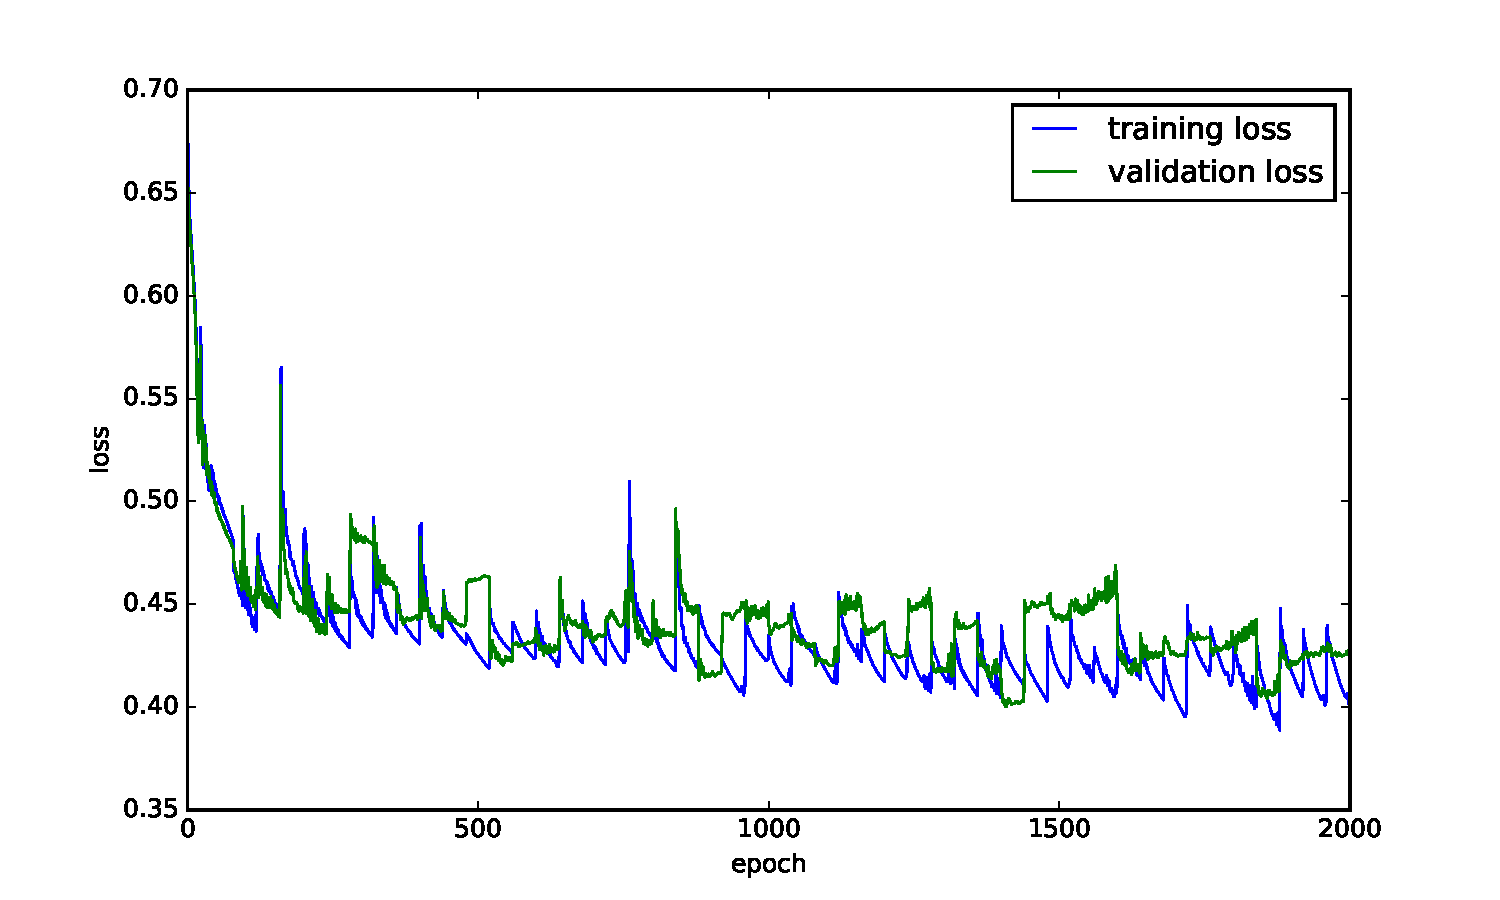
\includegraphics[width =0.5\textwidth]{../RNN_out/lstm64_3layers_wo_IPIP2D/loss-history.pdf}\label{a}}	
    \subfloat[][]{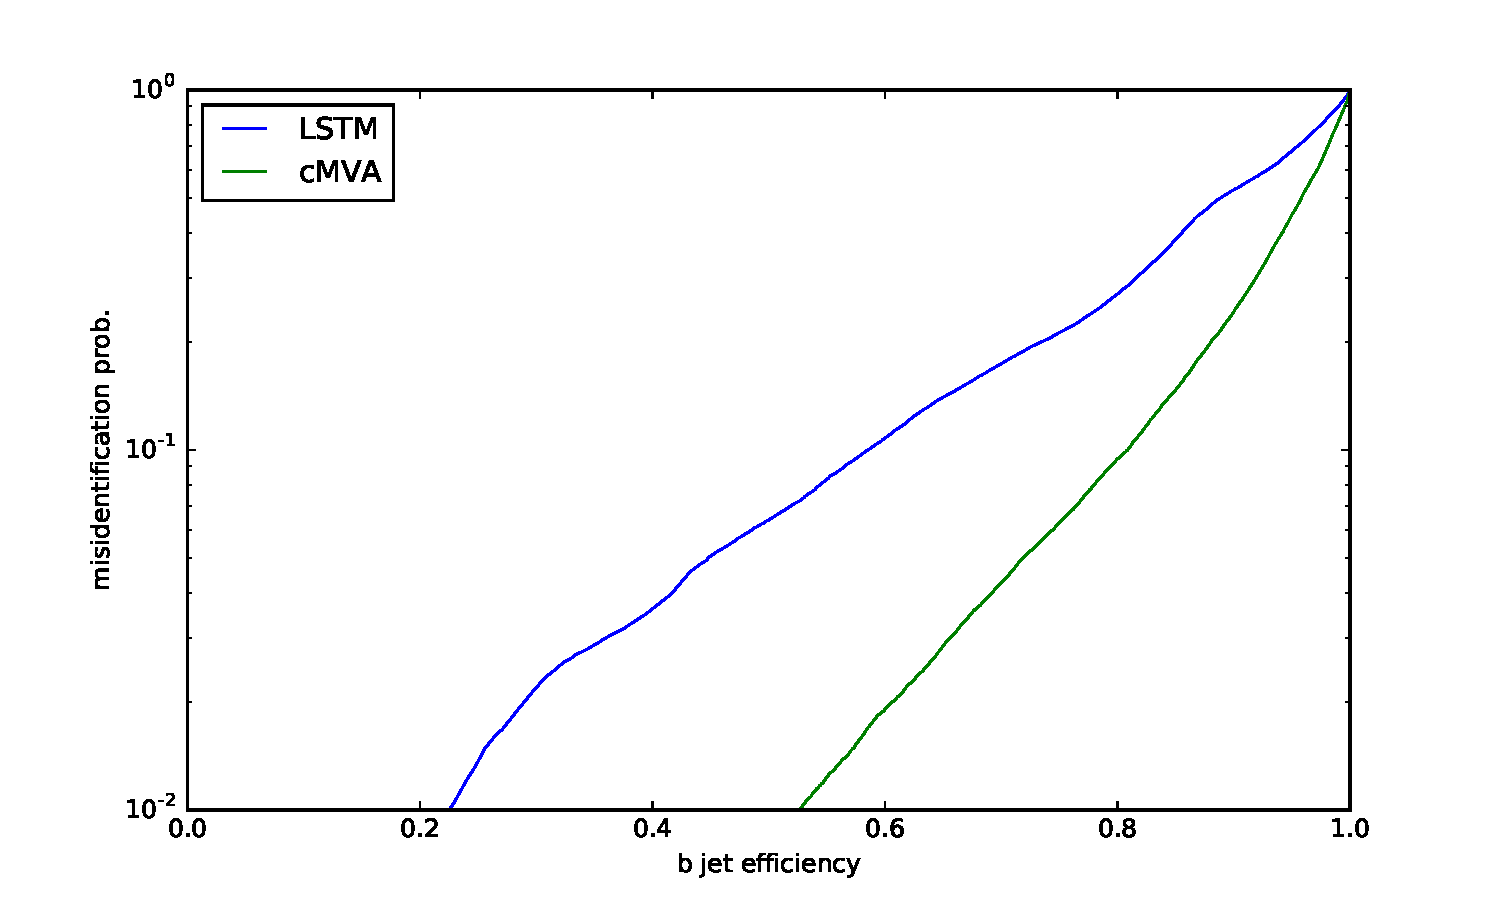
\includegraphics[width =0.5\textwidth]{../RNN_out/lstm64_3layers_wo_IPIP2D/ROC-plot.pdf}\label{b}}
  \end{figure}

  Performance \textsl{does} degrade!
  \begin{itemize}
  \item AUC(cMVA) = 0.9233
  \item AUC(LSTM) = 0.8368
  \end{itemize}
  
\end{frame}

\begin{frame}
  \frametitle{LSTM64 / 3: Training with reduced track parameters}
  \framesubtitle{without \texttt{Track\_eta} and \texttt{Track\_phi}}
  
  \begin{figure}
    \centering
    \subfloat[][]{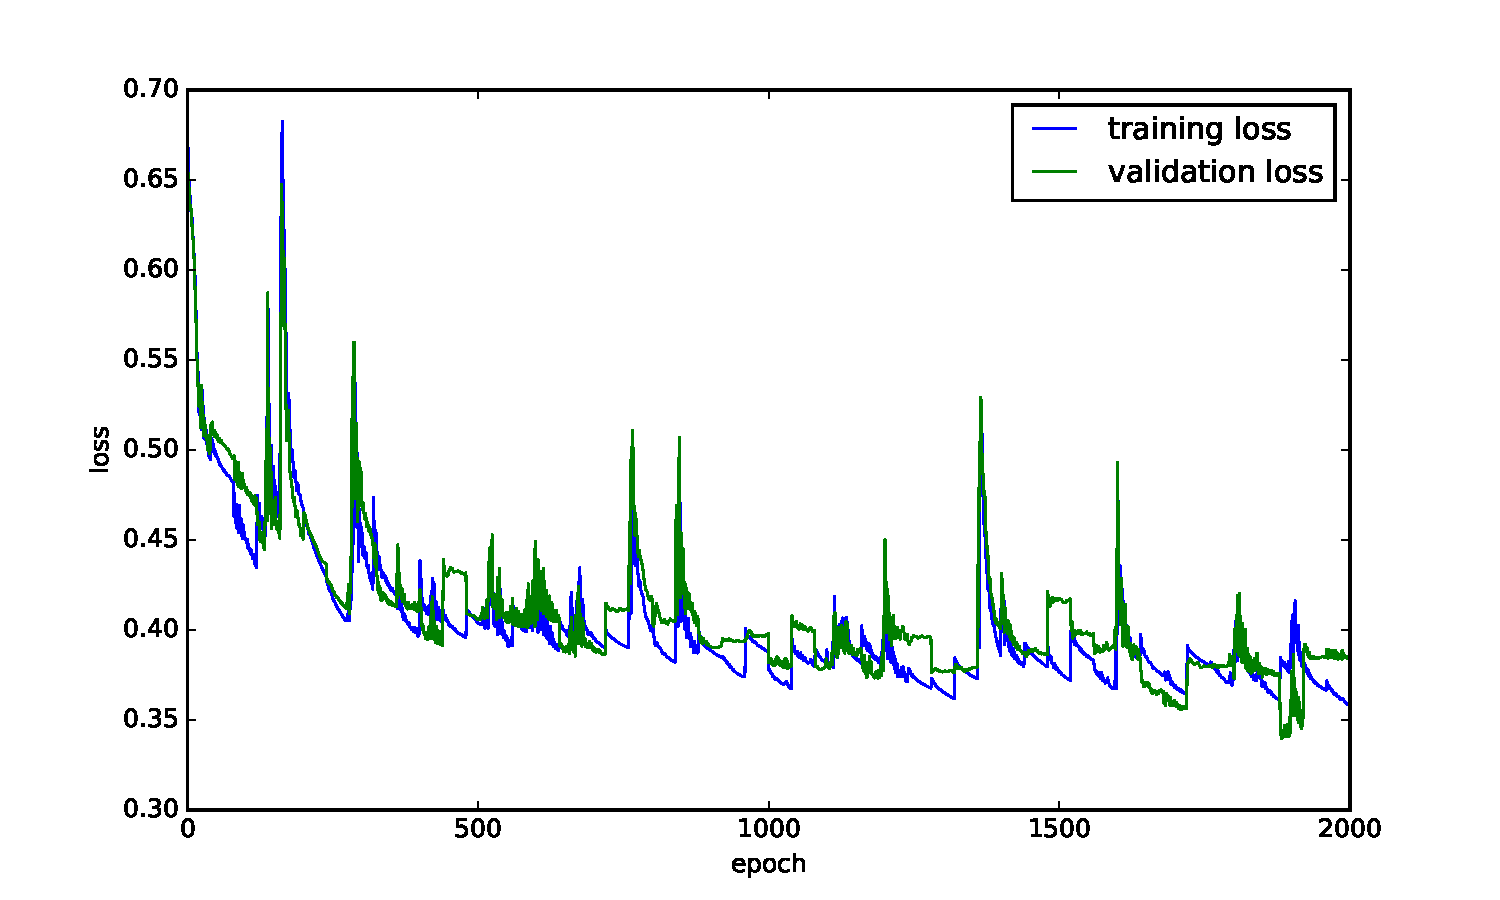
\includegraphics[width =0.5\textwidth]{../RNN_out/lstm64_3layers_wo_phieta/loss-history.pdf}\label{a}}	
    \subfloat[][]{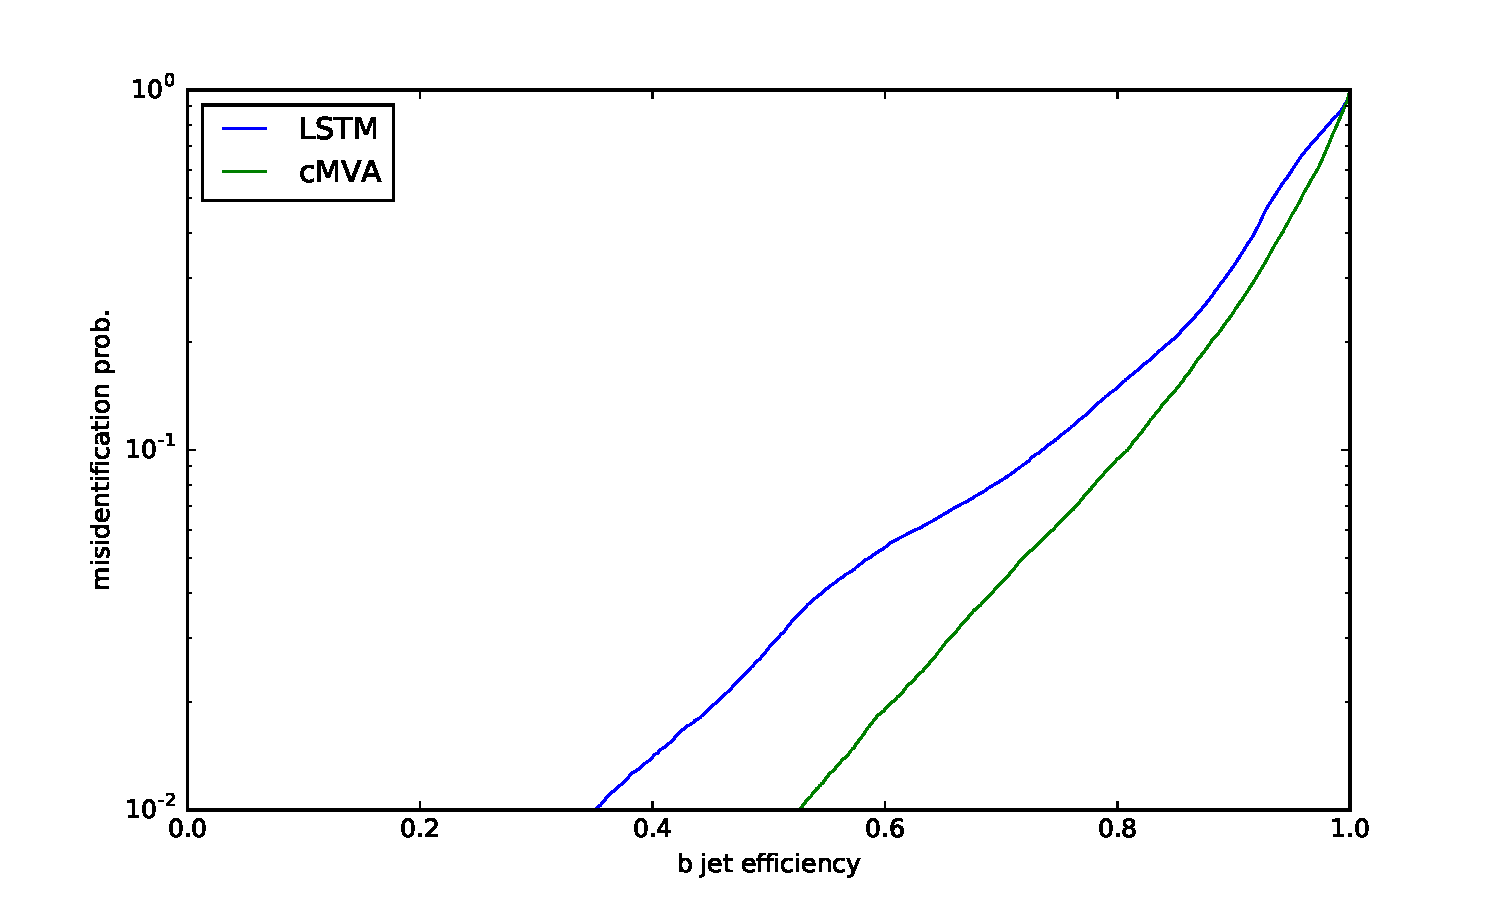
\includegraphics[width =0.5\textwidth]{../RNN_out/lstm64_3layers_wo_phieta/ROC-plot.pdf}\label{b}}
  \end{figure}

  Overall performance doesn't become worse, but the ROC curve is more chaotic $\leadsto$ less discriminative power in some kinematic regions?
  \begin{itemize}
  \item AUC(cMVA) = 0.9233
  \item AUC(LSTM) = 0.8922
  \end{itemize}
  
\end{frame}

\begin{frame}
  \frametitle{Conclusions}
  \begin{itemize}
  \item basic infrastructure seems to be in place and working
  \item classifier performance is very similar across the different networks that were evaluated
    \begin{itemize}
      \item training just not complete? Use still more epochs even if loss doesn't seem to improve much anymore?
      \item or is performance limited by the data representation / preprocessing rather than the network architecture?
    \end{itemize}
  \end{itemize}
\end{frame}

\begin{frame}
  \frametitle{Future Experiments}

  \begin{itemize}
  \item more sophisticated preprocessing?
  \item different representation (other than the raw track data)?
  \item try removing individual track parameters to see how performance degrades
  \end{itemize}
  
\end{frame}

\end{document}
